\chapter{因果响应}
\label{chap:causal-inference}

接受培训的人平均成绩更高，是培训提高了成绩，还是基础较好的人更愿意参加培训？
\BookChapterRef{chap:random-variables}{第~\ref{chap:random-variables}章}已经建立条件分布，第~\ref{chap:statistical-inference}章研究有限观测下的统计推断，第
~\ref{chap:information-theory-and-statistical-geometry}章进一步比较分布及其对任务的
影响。但把成绩预测得很准，仍不能回答主动安排培训以后会发生什么。后一个问题要求
说明：改变的究竟是对已有记录的筛选，还是产生记录的机制。

本章研究因果响应及生成它的结构。响应把行动与个体背景映射为结果；生成结构进一步
说明这个整体映射由哪些局部关系和机制合成。我们以处理\(T\)、结果\(Y\)与处理前
信息\(X\)为共同例子，区分给定模型的计算、基于可观测分布的响应识别，以及有限记录支持的生成结构
推断。模型明确给定时，可以直接比较行动，也可以在得知某人的事实以后计算替代结果；
这不意味着有限观测记录已经证明该模型正确。反过来，有些平均响应可以由实验设计识别，而无须
唯一恢复每一个局部方程。

计算行动后果需要一套响应规则，它把处理值与个体背景映成结果。固定同一背景可以比较个体效应，对目标总体平均可以比较人群效应；获得某人的事实后，还要先更新对其背景的认识。完成这些模型内的计算，再检查观测、实验和机制假设是否足以确定答案。

响应规则也可以由局部生成方程逐步合成。无环结构给出求值次序，图保留各方程读取的变量；这些条件进一步支持调整与结构推断。计算、识别和估计因此有各自的输入：给定模型可算出结果，相容模型是否给出同一结果决定可识别性，有限记录则决定估计精度。
对固定的计算程序，也可以替换输入或中间读数后重新求值；这种程序内响应能检查输出怎样依赖所用信息，推广为现实行动的后果则还需要生成机制的依据。

\section{因果响应的表示}
\label{sec:causal-response-representation}

设同一人可以接受或不接受某项培训，我们希望计算两种安排下的成绩。培训方案、个体背景与测量时间共同决定所比较的结果。观测回归\(\mathbb E[Y\mid T=t,X=x]\)只描述自然进入处理组的人；主动安排培训还要说明哪项生成规则被替换。响应映射将这个行动约定连同背景一起写进计算。

\subsection{原因与背景的响应表示}
\label{sec:causal-observation-generation}

比较同一人的行动后果时，需要固定两种行动共同具有的背景。用\(t\)记处理值，用\(\bm u\)记这些背景因素，例如既有能力与未测量因素；可见协变量只可能记录其中一部分。模型\(M\)给出背景分布、自然运行规则以及允许替换的规则。这里假定每套规则都确定唯一结果，局部方程如何支持这一假定将在生成结构部分证明。

模型要生成的处理、结果等变量称为内生变量（endogenous variables），它们的取值由
模型内的规则决定；作为这些规则输入、在当前模型中不再解释其来源的背景称为外生
变量（exogenous variables）。以培训为例，若模型写出了“培训怎样由个人情况决定”“成绩怎样由培训和能力决定”，那么培训与成绩是内生变量；而天赋、家庭支持等没有再写出生成公式、只作为输入给定的因素就是外生变量。“内生”和“外生”说明变量相对于模型边界的位置：把模型边界往外推，原来的外生变量也可能被纳入模型而成为内生变量，
外生变量仍可有现实原因，彼此也可以相关。下面先用整体映射表示背景如何生成状态，
第~\ref{sec:causal-local-structural-equations}节再把整体映射展开为局部方程。

\begin{definition}[因果响应与自然、行动映射]
  \label{def:causal-response-interface}
  给定背景可测空间\((\mathcal U,\mathscr U)\)及概率测度\(P_{\bm U}\)，
  自然变量的可测状态空间\(\mathcal V\)，以及可测的处理空间\(\mathcal T\)和结果空间
  \(\mathcal Y\)。状态空间包含处理、结果及其他内生坐标，并配有可测坐标映射
  \(\pi_T:\mathcal V\to\mathcal T\)、\(\pi_Y:\mathcal V\to\mathcal Y\)。
  固定模型\(M\)提供唯一值的可测自然映射
  \(F_M:\mathcal U\to\mathcal V\)，以及每个允许行动\(a\)的唯一值可测映射
  \(F_M^a:\mathcal U\to\mathcal V\)。后者由模型指定的机制替换产生，而非任意另选函数。
  若\(a(t)\)表示将处理生成规则替换为常量\(t\)的允许行动，
  即\(\pi_T(F_M^{a(t)}(\bm u))=t\)，则
  \term{因果响应}（causal response）是映射
  \begin{equation}
    R_M:\mathcal T\times\mathcal U\longrightarrow\mathcal Y,
    \qquad
    R_M(t,\bm u)=\pi_Y\bigl(F_M^{a(t)}(\bm u)\bigr).
    \label{eq:causal-response-interface}
  \end{equation}
  本章要求\(R_M\)对乘积可测结构可测。自然变量为
  \(\bm V=F_M(\bm U)\)，行动后的变量为\(\bm V_a=F_M^a(\bm U)\)。
\end{definition}

固定\(\bm u\)时，\(t\mapsto R_M(t,\bm u)\)回答同一单位怎样响应不同处理；
让\(\bm U\)按\(P_{\bm U}\)变化，才得到总体响应分布。外生背景的各分量可以相关，
定义没有默许独立性。若采用有限维参数表示\(M_{\bm\theta}\)，参数
\(\bm\theta\)描述研究者选定的机制；修改拟合参数是在改变模型，设置\(t\)则是在一个
固定模型内行动。两种变化不能互相代替。

下面用两套二元机制计算这一区别。设背景满足
\[
  U\sim\operatorname{Bernoulli}(1/2).
\]
处理与结果均取\(0,1\)。模型甲为
\begin{equation}
  T=U,\qquad Y=U;
  \label{eq:causal-observational-equivalence-confounding}
\end{equation}
模型乙为
\begin{equation}
  T=U,\qquad Y=T.
  \label{eq:causal-observational-equivalence-effect}
\end{equation}
两者自然映射都是\(F_M(u)=(u,u)\)，从而
\[
  \begin{aligned}
    \mathbb P(T=0,Y=0)&=\mathbb P(T=1,Y=1)=\frac12,\\
    \mathbb P(T=0,Y=1)&=\mathbb P(T=1,Y=0)=0.
  \end{aligned}
\]
在甲中，处理不进入结果规则；在乙中，结果直接复制处理。若允许的行动是把处理规则
替换为常数\(t\)，保留结果规则，则
\[
  F_{M_{\text{甲}}}^{a(t)}(u)=(t,u),\qquad
  F_{M_{\text{乙}}}^{a(t)}(u)=(t,t),
\]
所以\(R_{M_{\text{甲}}}(t,u)=u\)，而
\(R_{M_{\text{乙}}}(t,u)=t\)。两模型的自然映射相同，行动映射不同；
观测记录无法仅凭样本量区分这种差异。

图~\ref{fig:causal-identical-observation-different-intervention}把共同的观测规律只画一次，再并列画出同一行动后的两张结果分布。在自然记录中，\(T=1\)只会出现在\(U=1\)的单位身上；把处理规则替换为\(T=1\)却没有把背景也固定成\(U=1\)。模型甲因而仍保留两类背景各占一半的结果，模型乙的结果则随所设处理全部变成\(1\)。缺少机制信息时，观测规律相同不能决定应该使用右边哪张行动分布。

\begin{figure*}[htbp]
  \centering
  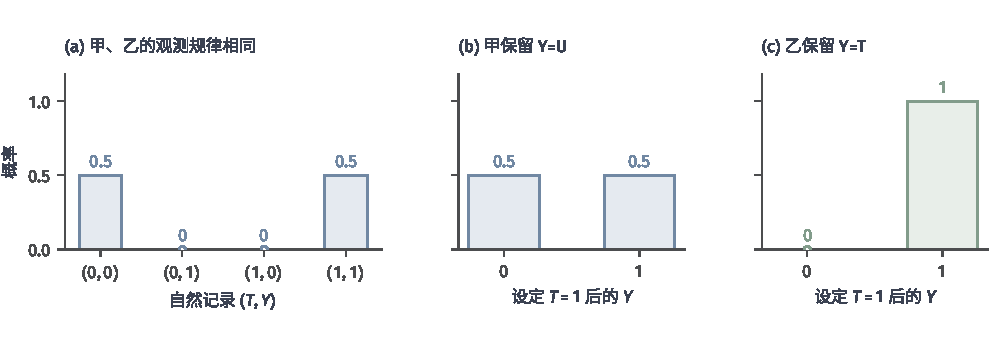
\includegraphics[width=169mm]{figures/00-shared/mathematical-preliminaries-lower/01-random-variables-distributions-and-causality/matplotlib/causal-identical-observation-different-intervention/figure.pdf}
  \caption{相同自然记录与不同的干预响应。背景\(U\sim\operatorname{Bernoulli}(1/2)\)，两模型都有\(T=U\)，但甲的结果规则为\(Y=U\)，乙为\(Y=T\)。左图给出两模型共同的自然联合概率；中、右图均把处理规则替换成\(T=1\)，分别保留各自的结果规则。所有柱高是给定教学机制的精确总体概率，共用概率尺度；中、右两图不是从左图按\(T=1\)筛选得到的条件分布。}
  \label{fig:causal-identical-observation-different-intervention}
\end{figure*}

\subsection{机制干预下的潜在结果}
\label{sec:causal-intervention-potential-outcomes}

在二元例子中，行动直接把\(T=U\)换成\(T=t\)，并沿用原来的结果规则。这项替换就是机制干预：它规定处理如何产生，再让保留的规则使用新的处理值。相同的观测条件概率没有记录这项替换，因此干预需要单独的模型约定。

\begin{definition}[理想干预]
  \label{def:causal-intervention}
  对给定模型的处理变量\(T\)作\term{干预}（intervention）
  \(\operatorname{do}(T=t)\)，表示删除自然生成\(T\)的规则，并以常量规则
  \(T=t\)替换。其余生成规则和指定的背景分布\(P_{\bm U}\)保持不变。
  由行动映射\(F_M^{a(t)}\)推前得到的分布记作
  \(P^{\operatorname{do}(T=t)}\)。
\end{definition}

“其余规则不变”不是说其余变量的取值不变。理解这一点的关键是：干预替换的是“处理怎样产生”这一条规则，而不是把其他变量的当前值冻结；所有以处理为输入的下游变量都要拿着新的处理值按各自原规则重新算一遍。若培训改变技能，技能再影响成绩，
行动后技能和成绩都应重算。只锁住所有非处理字段再评估一个预测器，通常不是这一行动。
多变量行动同样由\(F_M^a\)表达，但模型必须说明哪些规则替换、哪些保留。

干预已经确定怎样替换规则。现在仍从同一个背景总体分布抽取一个单位，并在所抽背景上执行指定处理，所得结果就成为一个随机变量。对同一单位比较两项处理时，两次计算必须复用同一个背景，才能表示这个单位本会得到的两种结果。
\begin{definition}[潜在结果]
  \label{def:causal-potential-outcomes}
  对明确的目标总体、处理版本和结果测量时间，\term{潜在结果}
  （potential outcome）是随机变量
  \begin{equation}
    Y(t)=R_M(t,\bm U).
    \label{eq:causal-response-potential-outcome}
  \end{equation}
  对二元处理，\((Y(0),Y(1))\)定义在同一背景概率空间上；两项分别表示同一单位
  在两种处理下的结果，而不是分别抽取两个人。
\end{definition}

这里的关键是“同一单位、两种安排”的对比：\(Y(1)\)和\(Y(0)\)是同一个人在两种平行情形下本会取得的成绩，二者之差才干净地反映培训对这个人的作用；如果拿参加培训的一群人和另一群没参加的人比，差异里还混着两群人本来的基础差距。
可测性保证可以讨论潜在结果的概率规律。记\(\mathcal L(Z)\)为随机变量\(Z\)的分布，
则
\[
  \mathcal L(Y(t))
  =
  (R_M(t,\cdot))_{\#}P_{\bm U}
  =
  \mathcal L(Y\mid\operatorname{do}(T=t)).
\]
符号\(\#\)表示\BookSectionRef{sec:rv-pushforward}{第~\ref{sec:rv-pushforward}节}的分布推前。这里的
\(\operatorname{do}\)标记修改后的模型，不是对自然事件\(T=t\)作普通条件化。
潜在结果聚焦所选行动下的输出；仅有一张潜在结果表，并不自动给出其他变量的完整
生成机制\scite{math-hernan2020whatif}

观察条件分布\(p(y\mid T=t)\)会筛选自然规则恰好给出处理\(t\)的单位，因而同时
包含处理作用和进入处理组的选择。在上面两套机制中，都有
\[
  \mathbb P(Y=1\mid T=1)=1,\qquad
  \mathbb P(Y=1\mid T=0)=0.
\]
但对甲，设定处理以后结果仍为\(U\)，故
\[
  \mathbb P(Y=1\mid\operatorname{do}(T=t))=\frac12,
  \qquad t\in\{0,1\};
\]
对乙，设定处理以后结果为\(t\)，故
\[
  \mathbb P(Y=1\mid\operatorname{do}(T=t))=t.
\]
相同的观测关联对应不同的行动后果。缺少的是关于响应机制的约束，不是更精确地估计
已经相同的两个条件概率。

固定处理值并非唯一行动。\term{随机干预}（stochastic intervention）用新的随机
规则替换处理规则，例如给定处理前信息\(X=x\)时，按概率核\(q(\cdot\mid x)\)安排培训。
这里\(q\)是从信息空间到处理空间的可测概率核。若这两个空间均为标准Borel空间，
可以加入独立于原背景的\(W\sim\operatorname{Unif}(0,1)\)，选取可测函数\(g_q\)，
使\(T=g_q(X,W)\)在给定\(X\)后的分布为\(q(\cdot\mid X)\)，再运行保留的机制。
有限处理空间中，这个构造就是按\(q\)的累计概率划分\([0,1]\)，读取\(W\)落在哪一段；
一般标准Borel空间则由概率核的随机化表示保证这样的可测实现。
若不满足这些空间条件，应直接以概率核的替换定义干预，不默认已有函数\(g_q\)。
确定性策略是新规则不再需要随机化的特例。随机化是否独立、行动可使用哪些信息，
都是干预定义的一部分；仅把某个概率因子改写为\(q\)不能保证其余现实机制未变。
局部机制成立时相应的分解公式在第~\ref{sec:causal-mechanism-composition}节建立。

\subsection{观测结果与干预响应的连接}
\label{sec:causal-response-observation-link}

一名接受培训的人的实际成绩，能否作为\(Y(1)\)的记录，取决于潜在结果所指的培训方案是否与实际执行一致。不同课程、时长和测量日期会给出不同的结果变量；先把这些条件固定，才能把记录接到相应的潜在结果上。对多名参与者，还要说明一人的处理是否会改变其他人的成绩。

这两项要求各管一件事。第一项要保证“\(Y(1)\)”这一记号指的是这个人实际接受的那种培训，
而不是另一种同名却内容不同的方案；若记录中的\(T=1\)对应的课程与潜在结果定义时的
课程不一致，两者就无法接到一起。第二项要保证一个人的成绩不受其他人处理的影响，
否则\(Y_i\)还要依赖整组人的处理安排，只比较\(t_i\)就不足以概括后果。
下面的定义把这两点分开写出。

\begin{definition}[处理一致性与无干扰]
  \label{def:causal-consistency-no-interference}
  对明确的处理版本，\term{一致性}（consistency）要求实际处理对应的结果满足
  \(Y=Y(T)\)几乎必然成立；特别地，
  \begin{equation}
    \begin{gathered}
      T=t\Longrightarrow Y=Y(t),\\
      \text{二元处理且结果为实数或实向量时，}\quad Y=TY(1)+(1-T)Y(0).
    \end{gathered}
    \label{eq:causal-consistency}
  \end{equation}
  对\(n\)个单位，无干扰要求：每个\(i\)及任意两个处理向量
  \(\bm t,\bm t'\)，只要\(t_i=t_i'\)，就有
  \(Y_i(\bm t)=Y_i(\bm t')\)几乎必然成立。因此单位\(i\)的潜在结果才可简记为
  \(Y_i(t_i)\)。
\end{definition}

一致性连接自然记录与行动响应，没有把未采取行动的结果变成可见记录。若模型给出
自然处理\(T=F_{M,T}(\bm U)\)，这一条件要求自然结果与
\(R_M(F_{M,T}(\bm U),\bm U)\)相合；不能任意拼接不相容的自然函数与响应族。
在依规则替换而构造的无环模型中，这种相合性可以逐方程检查。

无干扰则限制研究单位之间的相互作用。疫苗接种、社交网络和市场竞争中，一人的行动
可能改变他人的暴露或机会；此时\(Y_i(\bm t)\)往往依赖整个处理向量。
例如\(Y_i(\bm t)=t_i+\eta\sum_{j\ne i}t_j/(n-1)\)在
\(n>1,\eta\ne0\)时不满足无干扰。可以另行规定网络暴露、分组方案或总体处理比例，
但不能继续把只比较\(t_i\)的效应解释为所有联动后果。

通常所说的稳定单位处理值假设把处理版本唯一性和无干扰合在一起。它们与分配机制仍
须分开判断：分配机制规定\(T\)怎样依赖\(X,Y(0),Y(1)\)等量，一致性只连接实际
处理与观察结果。即使处理版本清楚且单位互不干扰，主动选择培训的人也可能具有不同
背景。响应的表示到此已建立，能否由这种选择后的观测恢复响应，是后面识别部分的问题。

\section{因果响应的比较与变化}
\label{sec:causal-response-comparison}

培训对不同人的作用可能方向相反，平均成绩也可能掩盖低分概率的变化。比较之前需要确定查询：同一人改变处理会差多少，对目标人群平均会差多少，还是结果分布某个部分会怎样移动。下面固定模型、处理版本与总体，分别给这些比较建立量；连续剂量的导数再说明当前剂量附近的小变化。

\subsection{同一背景下的响应比较}
\label{sec:causal-individual-response}

已经给定\(R_M\)时，计算同一人的两种结果只改变处理值\(t\)，背景\(\bm u\)保持不动。对实值成绩，可以直接相减；所得差值刻画这一背景下的处理作用，而不是两名不同人的成绩差。

\begin{definition}[同一背景下的响应差]
  \label{def:causal-individual-effect}
  对实值结果及允许的处理值\(t,t'\)，固定背景\(\bm u\)的响应差定义为
  \begin{equation}
    \Delta_M(t,t';\bm u)=R_M(t,\bm u)-R_M(t',\bm u).
    \label{eq:causal-individual-response-difference}
  \end{equation}
  二元处理的\term{个体处理效应}（individual treatment effect）是随机变量
  \(Y(1)-Y(0)=\Delta_M(1,0;\bm U)\)。
\end{definition}

这里的减法保持同一背景，而不是用一个处理组成员减去另一个未处理组成员。
例如\(R_M(t,u)=u+(2u-1)t\)，其中\(u\in\{0,1\}\)。对背景\(u=1\)，处理使
结果增加\(1\)；对\(u=0\)，处理使结果减少\(1\)。比较两名不同背景个体的实际
结果，还混入了基础值\(u\)的差异。

给定模型和背景时，两个响应都可以计算。但现实中一个人在同一时刻只能真实处在一种处理下，因此每个单位的实际记录只能包含
\(Y(T)\)，不会同时包含同一时刻的\(Y(1)\)与\(Y(0)\)：参加了培训就看不到他“假如没参加”的成绩，反之亦然。这就是因果推断里常说的“因果推断的根本难题”。因此“个体效应有明确定义”
与“它能由该人的一次观察确定”是两件事。即使已知某人当前结果为零，仍需要机制或
关于背景的信息才能计算另一行动下的结果。

对向量结果，可以先报告各坐标差，也可以指定具有实质含义的效用函数
\(h:\mathcal Y\to\mathbb R\)，比较
\(h(R_M(t,\bm u))-h(R_M(t',\bm u))\)。对类别结果，直接相减通常没有意义，
可以比较某事件的指示量。选择\(h\)是在规定目标，不是纯粹的记号替换：
提高收入、降低风险和同时满足两项要求，可能给出不同的行动排序。

\subsection{背景总体下的响应比较}
\label{sec:causal-population-response}

如果目标是决定一项培训是否适用于指定人群，两项行动都应按目标人群的同一个背景分布平均。这样得到的是总体作用，允许不同背景的个体效应互相抵消。保留完整结果分布还能看到均值没有显示的变化，例如成绩的尾部或分位数；两种报告服务于不同决策问题。

\subsubsection{总体与条件总体的平均响应比较}
\label{sec:causal-average-response}

个体效应\(Y(1)-Y(0)\)因人而异，决策者通常看不到也不需要每个人的确切效应，而是关心“对目标人群平均而言，培训值不值得推广”。把所有人在两种安排下的平均成绩相减，就得到这个总体尺度；计算时仍须让两种平均使用同一批人的背景分布，而不是比较两群不同的人。
\begin{definition}[平均处理效应]
  \label{def:causal-average-treatment-effect}
  对二元处理，假设\(Y(0),Y(1)\)都可积，\term{平均处理效应}
  （average treatment effect, ATE）定义为
  \begin{equation}
    \tau
    =
    \mathbb E[Y\mid\operatorname{do}(T=1)]
    -
    \mathbb E[Y\mid\operatorname{do}(T=0)].
    \label{eq:causal-ate-interventional}
  \end{equation}
\end{definition}

两个干预总体使用同一个\(P_{\bm U}\)。由潜在结果与干预分布的对应关系及期望线性性，
\begin{equation}
  \tau
  =\mathbb E[Y(1)-Y(0)]
  =\mathbb E[Y(1)]-\mathbb E[Y(0)].
  \label{eq:causal-ate-potential-outcomes}
\end{equation}
可积性排除了\(\infty-\infty\)这样的未定义运算。线性期望说明计算平均差只需要两个
边缘均值，并没有使同一单位的两个结果同时可见。上例若
\(\mathbb P(U=1)=\mathbb P(U=0)=1/2\)，ATE为零，但没有人的个体效应为零。

总体平均把受益和受损的人抵消成一个数，可能掩盖“培训对某类人特别有效、对另一类人无效甚至有害”。若要辨认哪些人可能受益、从而因人而异地安排处理，可以在处理前协变量\(X\)下分层，只对具有相同可观测特征的人平均效应。
\begin{definition}[条件平均处理效应]
  \label{def:causal-conditional-average-effect}
  设\(X\)在所比较干预下保持同一取值与含义，且两种潜在结果可积。
  \term{条件平均处理效应}（conditional average treatment effect, CATE）是
  \begin{equation}
    \tau(x)=\mathbb E[Y(1)-Y(0)\mid X=x],
    \qquad P_X\text{几乎处处}.
    \label{eq:causal-cate}
  \end{equation}
\end{definition}
它对具有相同已知特征的人平均，不等于这些人逐个具有相同效应。取
\(X=U\)时，上例的\(\tau(1)=1,\tau(0)=-1\)；若\(X\)未包含\(U\)，
条件平均仍可能掩盖层内差异。不能把处理后的技能水平直接当作这里不随行动变化的
\(X\)：按两种行动各自产生的技能筛人，通常不是比较同一条件总体。

全期望给出\(\tau=\mathbb E_X[\tau(X)]\)。若响应机制不变而目标总体从\(P_X\)
换为\(Q_X\)，且对应的条件背景规律与条件效应保持不变，新ATE为
\(\int\tau(x)Q_X(\mathrm dx)\)。这是人群权重的变化，不是机制突然发生改变；
条件效应能否跨总体保留本身仍需假设。目标总体、处理版本或测量时间改变，都应重新
标明效应的含义。

对有限处理集合\(\mathcal T\)，同样定义
\[
  \tau(t,t')=\mathbb E[Y(t)-Y(t')].
\]
若行动由处理前信息决定，则要比较整个策略。本段把同一处理\(T\)的允许取值组成
有限动作集合\(\mathcal A\subseteq\mathcal T\)，用处理值\(a\)标记“设定\(T=a\)”
这项行动。因此这里的\(Y(a)=R_M(a,\bm U)\)沿用潜在结果的定义；本段尚未把
\(a\)扩展为同时替换多项机制的一般行动。仍假定\(X\)不随这些处理行动改变。
策略\(\pi(a\mid x)\)用独立于原背景的新增随机化，在给定\(X=x\)时选择处理值\(a\)。
将\(\pi\)在\(\mathcal T\setminus\mathcal A\)上延拓为零，表示策略不会选择这些
处理值；这样以后即使对自然记录中的处理值求\(\pi(T\mid X)\)，记号也有定义。
在所有潜在结果可积时，它的单步价值为
\begin{equation}
  V(\pi)=\mathbb E_X\left[
    \sum_{a\in\mathcal A}\pi(a\mid X)\mathbb E[Y(a)\mid X]
  \right].
  \label{eq:causal-policy-value}
\end{equation}
式中独立随机化保证选择动作不会额外按未观测背景筛人。确定性策略是
\(\pi\)集中于一个动作的特例。这里定义的是给定模型内的目标；多值处理需要哪些
观测覆盖、策略可使用哪些已有记录，在第~\ref{sec:causal-effect-identification}节
再检查。连续剂量也不能被当作每个精确值都具有正概率的离散组。

\subsubsection{干预结果的分布响应比较}
\label{sec:causal-distribution-response}

平均值只记录分布的一个特征。设\(U\)等概率取\(-1,1\)，
\(Y(0)=0,Y(1)=U\)，则ATE为零，但处理后从人人得到零变成两种相反结果。
若低于零代表失败，未处理时的失败概率为\(0\)，处理后却为\(1/2\)。
均值虽相同，失败概率的变化仍会影响按风险选择行动的决策。

对实值结果，定义干预分布函数与其广义分位数
\[
  F_t(y)=\mathbb P(Y(t)\leq y),\qquad
  Q_t(p)=\inf\{y:F_t(y)\geq p\},\quad 0<p<1.
\]
\(F_t(y)-F_{t'}(y)\)比较不高于阈值的概率，\(Q_t(p)-Q_{t'}(p)\)比较两个总体
处于同一分位位置的结果。后者并不是个体效应
\(Y(t)-Y(t')\)的第\(p\)分位数，因为处于两个分布相同排名的未必是同一个人。
只有额外规定跨行动的排序对应关系，才能把这种配对解释成个体变化。

也可以使用第~\ref{chap:information-theory-and-statistical-geometry}章的分布比较
尺度。总变差比较事件概率而不要求矩；采用\(p\)阶Wasserstein距离时应满足所用
空间和有限\(p\)阶矩条件；使用KL散度则须检查绝对连续性及其值是否有限。
尺度的选择服务于所关心的风险或损失，不能用一个小均值差代替所有分布都接近。

两个干预边缘即使完全已知，仍没有说明它们如何在同一背景上配对。
第~\ref{sec:causal-factual-counterfactual}节将用两张联合表说明：分布比较足以回答
部分总体问题，却不足以回答已知某人事实结果后的替代结果。

\subsection{连续处理下的局部响应变化}
\label{sec:causal-local-response}

二元处理只能比较“做”与“不做”；当处理是药物剂量、培训时长、利率这类连续量时，还可以提出更细的问题：“在当前剂量上再增加一点点，结果大约改变多少？”这正是微积分里导数在因果响应上的对应物——它描述当前剂量附近的局部响应，而不是任意两个相差很大的剂量之差。
二元处理适合比较有无行动；连续剂量还可以询问“在当前剂量附近再增加一点会怎样”。
局部线性近似把小输入增量的响应写成线性主部与高阶余项；这里用它描述固定模型、
固定背景下的响应变化，而不是观测人群随剂量改变产生的回归变化。相关的可微性与
线性近似工具可参考
\BookChapterRef{chap:univariate-differentiation}{卷1《数学准备：计算、分析与几何》的“一元函数的微分”章}。

\begin{definition}[局部响应导数]
  \label{def:causal-local-response}
  设处理取值位于开集\(\mathcal T\subseteq\mathbb R^k\)，结果位于
  \(\mathbb R^m\)。用粗体标明向量剂量；若
  \(\bm t\mapsto R_M(\bm t,\bm u)\)在\(\bm t_0\)可微，其局部响应
  Jacobian为\(D_{\bm t}R_M(\bm t_0,\bm u)\)，满足
  \[
    R_M(\bm t_0+\bm h,\bm u)-R_M(\bm t_0,\bm u)
    =D_{\bm t}R_M(\bm t_0,\bm u)\bm h+o(\|\bm h\|).
  \]
  标量处理、标量结果时记为\(\partial_tR_M(t_0,\bm u)\)。
\end{definition}

该导数是每单位剂量的局部变化，不是任意有限剂量差。比如
\(R_M(t,u)=u+t^2\)，从\(t=1\)增加到\(1+h\)的响应差是\(2h+h^2\)，
局部导数为\(2\)。\(h\)很小时一阶项有用，但从\(1\)变到\(2\)的差为\(3\)，
不能直接用导数值\(2\)代替。离散行动没有这样的邻域，仍应使用有限差。

图~\ref{fig:causal-local-response-tangent}把这两个比较放在同一背景\(u=0\)下。切线只在\(t=1\)附近提供一阶近似；连接\(t=1\)与\(t=2\)的割线则累计了整个剂量区间内的响应变化。响应曲线弯曲时，割线斜率一般不等于起点处的导数。

\begin{figure}[htbp]
  \centering
  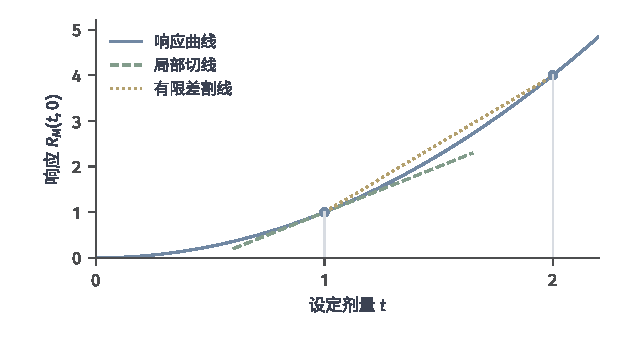
\includegraphics[width=105mm]{figures/00-shared/mathematical-preliminaries-lower/01-random-variables-distributions-and-causality/matplotlib/causal-local-response-tangent/figure.pdf}
  \caption{固定背景下的局部导数与有限剂量差。蓝实线为\(R_M(t,0)=t^2\)，绿虚线为\(t=1\)处斜率为\(2\)的切线；黄点线连接\((1,1)\)和\((2,4)\)，割线斜率为\(3\)。本例剂量差恰为\(1\)，所以有限响应差也为\(3\)；一般剂量差下还须除以剂量增量才得到割线斜率。}
  \label{fig:causal-local-response-tangent}
\end{figure}

总体平均响应\(m(t)=\mathbb E[R_M(t,\bm U)]\)还包含积分，不能仅凭每个人的
响应可微就交换求导与期望。下面给出一个可以直接检查的充分条件。
\begin{theorem}[平均响应的求导]
  \label{thm:causal-response-differentiation}
  设\(I\)是包含\(t_0\)的开区间，\(R_M(t_0,\bm U)\)可积。若对几乎每个
  \(\bm u\)，\(R_M(\cdot,\bm u)\)在\(I\)可微，且存在非负可积函数
  \(g(\bm U)\)，使
  \[
    |\partial_tR_M(t,\bm u)|\leq g(\bm u),
    \qquad t\in I,
  \]
  则\(m\)在\(t_0\)可微，且
  \begin{equation}
    m'(t_0)=\mathbb E[\partial_tR_M(t_0,\bm U)].
    \label{eq:causal-average-response-derivative}
  \end{equation}
\end{theorem}
\begin{proof}
  对足够小的非零\(h\)，中值定理给出
  \[
    \left|
      \frac{R_M(t_0+h,\bm u)-R_M(t_0,\bm u)}{h}
    \right|\leq g(\bm u).
  \]
  因而\(R_M(t_0+h,\bm U)\)可积，且差商几乎处处收敛到
  \(\partial_tR_M(t_0,\bm U)\)。可积的\(g\)统一控制这些差商，支配收敛定理
  允许将极限移入期望，得到
  \[
    \lim_{h\to0}\frac{m(t_0+h)-m(t_0)}{h}
    =
    \mathbb E\!\left[
      \lim_{h\to0}
      \frac{R_M(t_0+h,\bm U)-R_M(t_0,\bm U)}{h}
    \right],
  \]
  即所述结论。
\end{proof}

向量处理可以在相应可积控制下逐坐标求导；若要得到完整可微性，则需足以控制
Jacobian及余项的邻域条件。上述定理把“个体可微”与“可交换积分”分开，
后者限制少量背景下异常陡峭的响应，避免其破坏总体极限。

局部响应导数也不等于观测回归斜率
\(\partial_t\mathbb E[Y\mid T=t,X=x]\)。后者随\(t\)改变的还可能是自然进入
该剂量的人群。第~\ref{sec:causal-sensitivity-ranges}节以总体线性投影系数为例计算混杂偏差；这一系数一般也不等于上述逐点导数。
它同样不同于随机轨道的It\^o微分：这里对可设定输入作普通局部变化，背景固定；
随机轨道微分描述随时间累积的随机变化，一般不存在普通逐轨道时间导数。
因此模型的光滑性支持局部计算，却不同时保证这个导数能由观测识别或能外推到大幅行动。

\section{给定事实后的因果响应}
\label{sec:causal-counterfactual-recourse}

假设某人的处理、成绩和其他记录已经可见，我们希望判断另一行动会给他带来什么结果。此时不能重新从人群中抽取背景，因为事实已经排除了一些可能的背景。固定模型后，先由事实获得背景条件分布，再用替代行动映射同一组可能背景；反事实和行动补救都从这项条件化计算出发。

\subsection{事实条件下的反事实计算}
\label{sec:causal-factual-counterfactual}

给定事实\(\bm E=\bm e\)，所求对象是这个单位在替代行动下的条件结果。模型将自然记录与替代结果放在同一背景\(\bm U\)上，事实用于限定\(\bm U\)，行动用于改变生成规则；这两个操作需要分别保留。

\begin{definition}[给定响应模型的反事实变量]
  \label{def:causal-counterfactual}
  设模型\(M\)具有定义~\ref{def:causal-response-interface}的自然映射\(F_M\)及
  行动映射\(F_M^a\)。在同一外生背景\(\bm U\)上，\term{反事实}
  （counterfactual）变量定义为\(\bm V_a=F_M^a(\bm U)\)。
  给定实际证据\(\bm E\)后的反事实分布是\(\bm V_a\)关于该证据的条件分布，
  而不是重新按背景总体抽取一个人。
\end{definition}

事实证据可来自自然变量的一部分，也可包括带噪测量；后一情形把测量随机性一并纳入
背景，使证据的生成规则明确。反事实计算通常概括为三步——“溯因、干预、预测”，可以用一个例子体会：看到一名学生实际没参加培训却考了 70 分，先根据这个成绩反推他可能属于哪种能力水平（溯因，得到能力的条件分布）；再在脑海中把“是否参加培训”改成“参加”（干预，切换行动规则）；最后用更新后的能力和新规则重新推算他的成绩（预测）。
溯因由事实得到背景条件分布，干预切换到允许的行动映射，预测将同一个背景条件分布
推到结果空间。这里的溯因是给定模型内的条件化，并不是由一条记录证明模型正确。

设空间允许选取正则条件分布
\(P_{\bm U\mid\bm E=\bm e}\)，例如本章常用的标准Borel空间。按联合分布等于边缘分布与条件分布相乘的分解（离散与密度情形可参考\BookSectionRef{sec:rv-conditional-distribution}{第
~\ref{sec:rv-conditional-distribution}节}），对任意可测集合\(B\)，三步合成为
\begin{equation}
  \begin{aligned}
    \mathbb P(\bm V_a\in B\mid\bm E=\bm e)
    &=
    \bigl((F_M^a)_{\#}
      P_{\bm U\mid\bm E=\bm e}\bigr)(B)\\
    &=
    \int\mathbb I\{F_M^a(\bm u)\in B\}
      P_{\bm U\mid\bm E=\bm e}(\mathrm d\bm u).
  \end{aligned}
  \label{eq:causal-counterfactual-pushforward}
\end{equation}
式中事实只进入背景条件分布，行动只进入映射。连续证据点通常概率为零，等式按所选
正则条件分布版本理解，只保证对证据分布几乎处处的\(\bm e\)成立。在一个指定的
零概率证据点上报告数值，还需要选定版本或连续性等额外结构；积分恒等式本身不能
唯一规定每个点的条件值。

考虑已经明确给定的教学模型
\begin{equation}
  X=U_X,\qquad
  T=f_T(X,U_T),\qquad
  Y=2X+3T+U_Y.
  \label{eq:causal-counterfactual-linear-example}
\end{equation}
它直接提供自然映射及替换处理规则后的映射。某人的事实为
\(X=2,T=0,Y=5\)，于是
\[
  U_Y=5-2\times2-3\times0=1.
\]
保持该人的\(X,U_Y\)不变，把处理设为\(1\)，得到
\[
  Y_{T\leftarrow1}=2\times2+3\times1+1=8.
\]
差值\(3\)来自给定结果规则中的处理作用。事实不必确定全部背景，例如可能仍不知道
\(U_T\)；只要未确定部分不影响本次行动后的结果，仍能得到这个点值。
若结果规则不确定，或未确定的背景继续进入结果，则应给出条件分布或范围。

\begin{example}[两点背景后验的反事实推前]
  \label{ex:causal-two-point-background-posterior}
  令背景类型\(U\in\{u_{\mathrm L},u_{\mathrm H}\}\)先验概率各为\(1/2\)。
  事实中观察到二元信号\(S=1\)，且模型规定
  \[
    \mathbb P(S=1\mid U=u_{\mathrm H})=\frac34,\qquad
    \mathbb P(S=1\mid U=u_{\mathrm L})=\frac14.
  \]
  因而\(\mathbb P(S=1)=\frac12(\frac34+\frac14)=\frac12\)，Bayes公式给出
  \[
    \mathbb P(U=u_{\mathrm H}\mid S=1)=\frac34,\qquad
    \mathbb P(U=u_{\mathrm L}\mid S=1)=\frac14.
  \]
  若行动\(a\)下的结果在两类背景中分别为
  \(F_{M,Y}^a(u_{\mathrm L})=2,F_{M,Y}^a(u_{\mathrm H})=6\)，则
  \[
    \mathcal L(Y_a\mid S=1)=\frac14\delta_2+\frac34\delta_6,\qquad
    \mathbb E[Y_a\mid S=1]=\frac14\,2+\frac34\,6=5.
  \]
  忽略事实而按先验重新抽取背景，得到总体干预分布
  \(\frac12\delta_2+\frac12\delta_6\)，均值为\(4\)。
  两个答案使用同一行动映射，只是反事实计算保留了事实提供的背景信息。
\end{example}

这个例子也可放回完整背景接口：另加独立测量随机量生成信号\(S\)，行动结果只依赖
类型\(U\)，于是积分掉测量背景就得到上面的两点后验。未知背景不必被硬选成某一类。

图~\ref{fig:causal-abduction-intervention-prediction}并列展示这两条推前路径：条件反事实保留事实形成的后验，总体干预沿用背景先验。

\begin{figure*}[htbp]
  \centering
  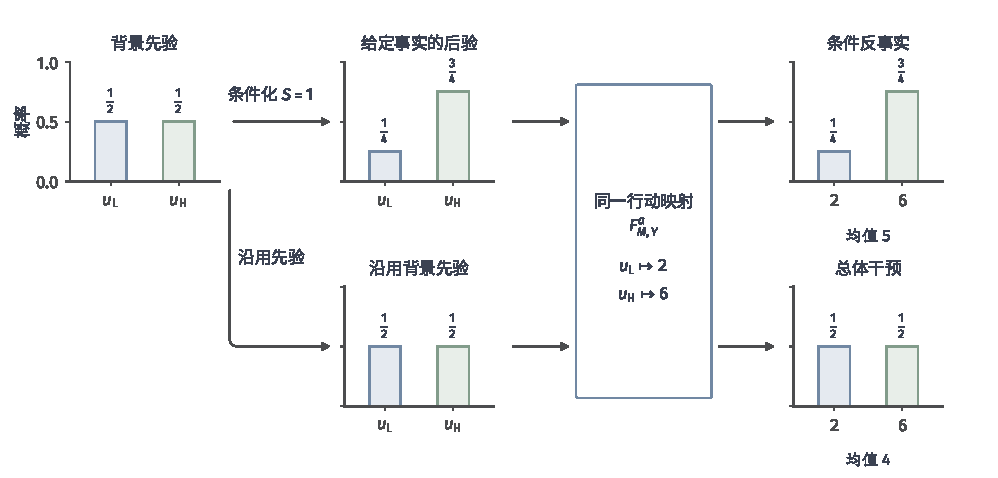
\includegraphics[width=169mm]{figures/00-shared/mathematical-preliminaries-lower/01-random-variables-distributions-and-causality/matplotlib/causal-two-point-pushforwards/figure.pdf}
  \caption{同一行动映射下的条件反事实与总体干预。背景$u_{\mathrm L},u_{\mathrm H}$的先验概率各为$1/2$，
  事实$S=1$将两者的后验概率更新为$1/4,3/4$；行动映射分别给出结果$2,6$。
  保留后验得到条件均值$5$，沿用先验得到总体干预均值$4$。
  概率柱使用共同的零基线与比例尺；溯因是给定模型内的条件化，不证明结构假设本身有效。}
  \label{fig:causal-abduction-intervention-prediction}
\end{figure*}


还有一种更深的歧义：即使知道两种行动各自的总体分布，也未必知道同一个人的两个
结果怎样配对。设两种干预结果均为\(\operatorname{Bernoulli}(1/2)\)。
模型甲令一半单位满足\((Y(0),Y(1))=(0,0)\)，另一半满足\((1,1)\)；
模型乙令两类单位分别满足\((0,1)\)和\((1,0)\)。甲的个体效应恒为零，
乙的个体效应等概率取\(1,-1\)，而两模型的ATE都为零。

图~\ref{fig:causal-cross-world-couplings}给出了对应的联合概率表。用定义
~\ref{def:information-coupling}的语言，两者是相同边缘的不同耦合。
已知\(Y(0)=0\)时，甲给\(Y(1)=0\)，乙给\(Y(1)=1\)。在独立随机分配处理
的事实世界里，把同一事实\(T=0,Y=0\)分别输入两套模型，会得到不同的条件反事实。
这项计算比较的是模型给出的答案，并没有用该事实区分两套模型。

\begin{figure}[htbp]
  \centering
  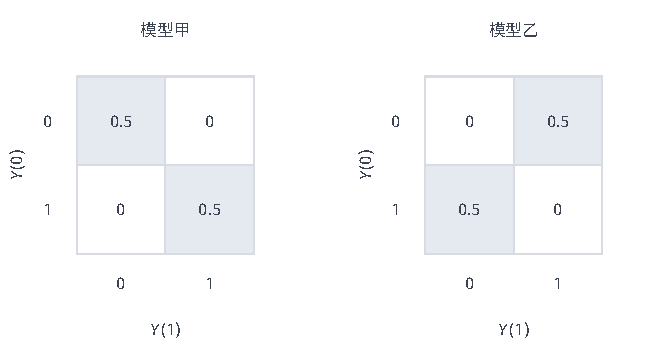
\includegraphics[width=\linewidth]{figures/00-shared/mathematical-preliminaries-lower/01-random-variables-distributions-and-causality/tikz/causal-cross-world-couplings/figure.pdf}
  \caption{相同干预边缘的两种跨世界配对。行对应\(Y(0)\)，列对应\(Y(1)\)，格内
  数字为联合概率；每张表的行和、列和均为\(1/2\)。甲的个体效应恒为零，乙的个体
  效应等概率取\(1,-1\)，两者ATE均为零。这是相容机制的教学构造，不是随机试验
  直接观察到的潜在结果联合表。}
  \label{fig:causal-cross-world-couplings}
\end{figure}

两套配对连完整随机试验的两组边缘也无法区分。要回答条件个体反事实，还需要关于
跨世界联合结构的机制限制，或具有适当稳定性、时间和携带效应假设的重复干预资料；
否则应保留相容范围。模型明确给定时可以用式
~\eqref{eq:causal-counterfactual-pushforward}计算，可观测分布与机制假设是否足以确定这套模型则是
第~\ref{sec:causal-effect-identification}节的另一个问题。

\subsection{目标约束下的行动补救}
\label{sec:causal-action-recourse}

反事实计算还可以反过来服务于行动选择：当模型预测某人会被拒绝（比如贷款申请未通过），他自然想问“我该做些什么才能通过审核”，而这些改变应当是现实中真正能做到的。这就是行动补救要解决的问题——怎样以尽量低的代价，让同一个人的决策
达到目标？先要区分两种看似相近、实则不同的操作。对预测器\(\widehat y=f(x,t)\)，输入替换给出
\[
  f(x,1)-f(x,0).
\]
这只是已训练函数对字段变化的响应，相当于在计算器里把一个输入数字改掉再看输出，并不考虑现实中改变这个字段会牵动什么。若现实培训提高技能、同时占用工作时间，那么
只改“是否培训”一列而锁住技能和时间，通常不是任何可实施的行动结果。

\begin{definition}[因果行动补救]
  \label{def:causal-recourse}
  给定事实证据\(\bm E=\bm e\)，以\(x=\xi(\bm e)\)表示由事实确定的行动信息摘要，
  其中\(\xi\)为预先指定的可测映射。给定可实施行动集合\(\mathcal A(x)\)、响应模型、行动成本\(c(a;x)\)
  与目标决策集合\(G\)，\term{行动补救}（algorithmic recourse）寻找能够使行动后
  的决策落入\(G\)的可行行动。因果行动补救用同一背景下的干预状态
  \(\bm V_a=F_M^a(\bm U)\)评价成功条件，并按机制重算所有受行动影响的状态。
\end{definition}

令\(d\)为最终决策规则。若事实唯一确定背景\(\bm u\)，优化形式为
\begin{equation}
  \min_{a\in\mathcal A(x)}c(a;x)
  \quad\text{使得}\quad d(F_M^a(\bm u))\in G.
  \label{eq:causal-recourse-objective}
\end{equation}
可行集合规定实际允许做什么，成本规定如何比较行动，成功约束规定要得到何种决策。
这三项共同规定一个约束优化问题，不能只用一个距离函数代替。低输入距离不等于低行动成本；不可改变属性也不应成为行动建议。
若可行集合为空，应报告无法在当前约束下补救，而不是输出一个不可执行的最近点。
相关工具可参考\BookChapterRef{chap:optimization}{卷1《数学准备：计算、分析与几何》的“最优化”章}。

多数事实只能给出背景条件分布。给定可容许失败概率\(\alpha\in[0,1]\)，可以采用
概率型约束
\begin{equation}
  \mathbb P\bigl(d(F_M^a(\bm U))\in G\mid\bm E=\bm e\bigr)
  \geq1-\alpha.
  \label{eq:causal-recourse-probability}
\end{equation}
这个条件要求失败背景集合的后验概率至多为\(\alpha\)。回到例
~\ref{ex:causal-two-point-background-posterior}，若目标是\(Y_a\geq5\)，行动\(a\)
的后验成功概率为\(3/4\)，因此在\(\alpha=1/4\)时满足概率约束；但低类型背景的
结果为\(2\)，这一类仍与事实相容的背景全部失败。只挑高类型作为“代表背景”会
漏掉这项风险。

若要求每个保留下来的背景都成功，就需要比允许少量失败更强的逐点约束。为此先要
说明保留哪些背景。离散情形可保留每个具有正后验概率的背景；连续情形的单点可能
都是零概率，不能用单点概率判断是否应被保留。给背景空间配上拓扑后，可以保留
那些无论取多小邻域、邻域仍有正条件概率的点，这些点组成条件分布的支持。
若背景空间为Polish空间，且所用条件分布版本是其Borel概率测度，则可说明这个
支持为何覆盖条件概率一。Polish空间有可数拓扑基，
支持以外的点可被可数个零概率开集覆盖；因此支持是闭集且具有条件概率一。
记这个支持为
\[
  \mathcal S_{\bm e}
  =\operatorname{supp}P_{\bm U\mid\bm E=\bm e}.
\]
在这个候选背景集合上要求
\begin{equation}
  d(F_M^a(\bm u))\in G,\qquad \bm u\in\mathcal S_{\bm e},
  \label{eq:causal-recourse-robust}
\end{equation}
这给出支持上的最坏情形保证。该支持具有条件概率一，因此支持上的逐点成功蕴含概率一成功；它还约束支持中
零概率点上的模型取值，因而可能严格更强。一般可测空间没有默认的拓扑支持，
此时应明确给出候选背景集合。若要由该集合上的逐点保证推出概率一成功，
还须要求该集合具有条件概率一。

上面的两点后验支持同时包含高、低两类背景，所以同一行动虽然满足成功概率
\(3/4\)的要求，却不满足支持上的逐点保证。两种约束分别回答“允许多大失败概率”
和“是否覆盖每个保留背景”，应按所需保证选择，不能把前一种达标解释成后一种也达标。

补救也有时间和多人联动的边界。许多人同时接受建议可能改变价格、名额或审核规则；
决策系统更新后，原建议未必仍有效；资源竞争也可能使原先逐人可行的行动无法共同
执行。因此当前模型中存在一个成功行动，不等于建议已经通过现实可行性、持久性
或公平性验证。

\subsection{目标属性干预下的公平补救}
\label{sec:causal-fair-recourse}

设行动已经能改变当前决策，我们还可能要求这种成功不依赖某项受保护属性，例如性别或种族。属性可能经其他变量影响决策，所以只从预测字段中删除属性，并不能保证消除这些影响。给定同一份事实证据后，我们先得到对个体背景的条件分布，再分别改变属性并重新计算它所影响的变量，比较两个属性世界中的预测条件分布。背景全部固定时，两个预测值相同是更强的逐背景要求；下面的定义只要求在同一个事实背景条件分布下，两个预测分布相同，不要求每个未观测背景上的值都相同。哪些属性作用应被排除仍是一项规范选择；给定选择后，模型才规定具体的反事实比较。

令受保护属性为\(A\)，事实证据为\((X=x,A=a)\)。本小节的\(X\)泛指用于推断
背景的其他事实，可能包含属性的后继变量；它不再具有CATE中“处理前且保持不变”
的自动含义。事实中给定\(X=x\)，并不要求替代属性世界的\(X\)仍等于\(x\)。
\begin{definition}[反事实公平]
  \label{def:causal-counterfactual-fairness}
  在给定响应模型与预测规则下，\term{反事实公平}（counterfactual fairness）
  要求：对每个允许的替代属性\(a'\)和每个可测预测值集合\(B\)，以下等式对事实
  证据分布几乎处处的\((x,a)\)成立：
  \begin{equation}
    \begin{aligned}
      &\mathbb P(\widehat Y_{A\leftarrow a}\in B\mid X=x,A=a)\\
      &\qquad=
      \mathbb P(\widehat Y_{A\leftarrow a'}\in B\mid X=x,A=a).
    \end{aligned}
    \label{eq:causal-counterfactual-fairness}
  \end{equation}
  两个属性世界均使用同一个事实背景条件分布，并重新计算由属性影响的状态及预测。
\end{definition}

等式右侧仍以事实\(A=a\)为条件，而不是改用另一群人的证据\(A=a'\)。
只在输入表中替换\(A\)并固定其全部后继变量，检验的是另一个对象。属性干预在这里
是明确模型下的比较操作，也不表示应建议个人改变该属性。

把公平条件加入补救时，为避免与属性值混淆，记补救行动为\(b\)。
要求模型已经规定联合行动映射\(F_M^{b,A\leftarrow a'}\)：对每个属性世界，
保留同一个可比较的行动\(b\)，不对该世界偷偷重新选择更有利的行动。行动与属性
替换须互相兼容，且所比较世界中行动的可实施含义应明确。定义
\[
  \Pi_b^{a'}(B;x,a)
  =
  \mathbb P\bigl(
    d(F_M^{b,A\leftarrow a'}(\bm U))\in B
    \mid X=x,A=a
  \bigr).
\]
一种公平约束补救问题是
\begin{equation}
  \begin{aligned}
    \min_{b\in\mathcal A(x,a)}\quad &c(b;x,a)\\
    \text{使得}\quad
    &\Pi_b^a(G;x,a)\geq1-\alpha,\\
    &\Pi_b^{a'}(\cdot;x,a)=\Pi_b^a(\cdot;x,a)
      \quad\text{对每个允许的 }a'.
  \end{aligned}
  \label{eq:causal-fair-recourse-objective}
\end{equation}
第一项约束要求成功，第二项约束要求同背景的决策分布不随属性改变。也可以另选近似
公平或成本公平目标，但那会改变问题，不能把它们当作上述等式的自动结果。

\begin{example}[成功行动未必满足公平约束]
  \label{ex:causal-fair-recourse}
  设\(A\in\{0,1\}\)，自然培训量为\(B=0\)，资格分数与二元决策规则为
  \[
    K=U+A+B,\qquad d=\mathbb I\{K-2A\geq2\}.
  \]
  可行行动是把培训量设为\(b\in[0,3]\)，成本为\(c(b)=b\)，目标为\(d=1\)。
  已知事实\(A=0,B=0,K=1\)，于是\(U=1\)。在两个属性世界中施加同一行动，
  必须重算\(K\)，得到
  \[
    K_{b,A\leftarrow a'}=1+a'+b,\qquad
    d_{b,A\leftarrow a'}=\mathbb I\{1+b-a'\geq2\}.
  \]
  只要求事实属性下成功时，最小行动为\(b=1\)。但此时\(a'=0\)给决策\(1\)，
  \(a'=1\)给决策\(0\)，并不公平。若同时要求两个属性世界的二元决策相同且
  成功，则必须\(b\geq2\)，故最优行动为\(b=2\)。不行动时两个世界都失败，
  虽然决策相同，却不满足补救目标。
\end{example}

此例检验的是二元决策，不是内部实值分数\(K-2A\)；后者在两个属性世界中始终
相差\(1\)，任何培训量都不能让分数分布相同。公平对象、允许行动及预算都会影响
可行性。对一个已知个体成立的约束，也不自动保证面向所有人的推荐规则公平；
后者还需规定推荐怎样依赖事实，并对其目标人群几乎处处检验。

这些等式均以给定模型为条件。第~\ref{sec:causal-factual-counterfactual}节的
跨世界配对已经说明，相同干预边缘也可能给出不同条件反事实；由观测拟合出一套
生成规则，不等于公平或补救结论已被唯一识别。若多个模型与证据相容，应在该模型类
上报告结论范围。哪些属性或路径属于不应进入决策的因素，则是另需论证的规范选择。
公平要求、解释和行动补救还涉及应用中的现实验证边界，后续章节将继续讨论。
相关工具可参考\BookChapterRef{chap:trust-fairness}{卷3《基础、理论与可信性》第13章“公平性”}、\BookChapterRef{chap:trust-interpretability}{卷3《基础、理论与可信性》第15章“可解释性”}。

\section{因果响应的推断}
\label{sec:causal-effect-identification}

响应计算给出指定模型中的答案，实际研究却可能不知道哪套机制产生了观测。识别先固定可观测分布和机制假设，保留与两者相容的全部模型，再检查这些模型是否给出同一个响应目标。若相同可观测分布对应不同的培训效应，增加按同一制度采集的样本也不能消除该目标的歧义；若所有相容模型给出相同效应，目标才被识别。这里的“相同”指总体观测规律相同，不是两套模型都能产生某一批有限记录。后者仍可能具有不同观测分布，并随重复采样而被区分。把完整生成机制当作候选模型，就回到定义~\ref{def:statistics-identifiability}中的目标可识别性；目标已唯一确定后，再讨论有限样本的估计误差。

这里比较的是“完整生成机制”，不是拟合参数。两套机制可以有完全不同的结构方程和背景分布，
只要它们在已声明的观测制度下给出同一个可观测分布，观测资料就无法分辨它们。
可识别性问的正是：在这些无法分辨的模型之间，目标值是否已经一致。
若一致，说明资料足以确定目标；若不一致，增加同类样本只能把共同的可观测分布估得更准，
并不能消除这层歧义。

记\(P_{\mathrm{obs}}^M\)为模型\(M\)在已声明观测制度下给出的可观测分布，
\(\tau(M)\)为目标。在允许模型类中，若对任意两套模型\(M_1,M_2\)都有
\[
  P_{\mathrm{obs}}^{M_1}=P_{\mathrm{obs}}^{M_2}
  \quad\Longrightarrow\quad \tau(M_1)=\tau(M_2),
\]
就称该目标\term{可识别}（identifiable）。可观测分布可以包括已完成的试验资料，
不必只包括自然观察。目标可识别也不要求模型每个组成部分都唯一确定。

这是总体层面的唯一性，须与有限样本估计、数值计算区分。估计用样本逼近总体量，
计算求出给定表达式或优化问题的答案。一个算法可以精确拟合全部观测条件分布，
却仍无法区分本章开头的两套机制；反过来，目标已有识别式，也不表示样本够多或
数值算法已经稳定。

开篇式~\eqref{eq:causal-observational-equivalence-confounding}与式
~\eqref{eq:causal-observational-equivalence-effect}已经给出可核对的反例：两套模型
都有\(U\sim\operatorname{Bernoulli}(1/2)\)和\(T=U\)，但甲的结果规则为\(Y=U\)，
乙为\(Y=T\)。两者的自然记录都只有\((T,Y)=(0,0),(1,1)\)，概率各为\(1/2\)。
把同一个处理规则替换为\(T=t\)以后，甲仍有\(Y(t)=U\)，乙则有\(Y(t)=t\)，因此
\[
  \begin{aligned}
    \tau(M_{\text{甲}})&=\mathbb E[U-U]=0,\\
    \tau(M_{\text{乙}})&=\mathbb E[1-0]=1.
  \end{aligned}
\]
只要允许模型类同时保留这两套机制，平均效应就不可识别。它们不是仅有处理分配
不同：恰恰是结果机制不同，却在自然记录中表现相同。增加同类记录无法排除其中
任何一套，需要改变观测制度或加入能区分它们的机制假设。

反过来，找到某两套观测等价模型恰好给出相同目标，还不足以证明可识别。必须检查
允许模型类中所有产生同一可观测分布的模型；只有它们的目标均一致，资料才唯一
确定该目标，随后才讨论有限样本下能估得多准。判断某条识别式是否成立，应检查
它用到了哪些假设，而不是只看它能否在数据上算出数字。

\subsection{响应目标的点识别}
\label{sec:causal-point-identification}

目标处理下的结果只在实际得到该处理的人身上可见。要用他们代表目标总体，需要限制处理选择与潜在结果之间的关系。随机分配直接建立这种关系；观察研究可以在处理前信息充分时，用条件交换性支持调整。下面先在潜在结果语言中证明相应等式，再由图条件解释某些调整集合为何成立。

\subsubsection{随机分配下的边缘识别}
\label{sec:causal-randomized-identification}

若处理由独立随机装置分配，且两种处理都有正概率，则
\((Y(0),Y(1))\perp T\)。结合一致性，对任意可测集合\(B\)及
\(t\in\{0,1\}\)，有
\begin{equation}
  \mathbb P(Y(t)\in B)
  =
  \mathbb P(Y(t)\in B\mid T=t)
  =
  \mathbb P(Y\in B\mid T=t).
  \label{eq:causal-randomization-marginal-distribution}
\end{equation}
第一个等号来自随机分配，第二个来自实际处理与潜在结果的一致性；正概率保证右侧
有相应处理组。结果可积时，同一论证给出
\[
  \mathbb E[Y(t)]
  =\mathbb E[Y(t)\mid T=t]
  =\mathbb E[Y\mid T=t],
\]
所以两组均值差识别ATE。

式~\eqref{eq:causal-randomization-marginal-distribution}识别的是每个潜在结果的
完整边缘，不是\((Y(0),Y(1))\)的联合分布。第
~\ref{sec:causal-factual-counterfactual}节的两套配对因此仍与随机试验相容。
若实际分析存在失访、不依从、处理溢出或随机化后的样本筛选，应按真实目标重新检查
独立性和一致性。例如随机分配的邀请不等于实际参加培训，按参加者重新分组不会自动
继承原随机化。

\subsubsection{条件交换下的调整识别}
\label{sec:causal-adjustment-identification}

观察研究不能随意重排处理，分配是否参加培训往往由个人自己决定，但可以尝试用处理前\(X\)解释这种分配差异：只要把所有同时影响“是否参加”和“成绩”的处理前因素都纳入\(X\)，那么在这些因素相同的人中间，谁参加培训就可以看作近似随机。这里的\(X\)
须在所比较处理下保持同一取值和含义，否则两组不再按共同背景分层。
\begin{definition}[条件交换性]
  \label{def:causal-conditional-exchangeability}
  对二元处理，\term{条件交换性}（conditional exchangeability）要求
  \begin{equation}
    (Y(0),Y(1))\perp T\mid X.
    \label{eq:causal-conditional-exchangeability}
  \end{equation}
\end{definition}
直观上，固定\(X\)后，进入处理组不再额外透露潜在结果的信息；例如\(X\)已经
包含需要控制的共同背景。这不同于概率论中样本序列在重排下分布不变的可交换性。
它涉及不能同时观察的结果，不能凭处理预测准确率或结果拟合误差验证。对单个边缘
目标，只需相应的\(Y(t)\perp T\mid X\)；上式是同时表达两种处理可比性的较强条件。

即使处理前背景足以支持条件交换性，某一背景层的自然处理概率仍可能为\(0\)或\(1\)。例如某类高危患者按制度必须用药，该层就没有不服药的总体对照规律可由自然记录识别。交换性不会补出这种支持缺口，因此用两组条件均值比较时，还需两种处理在目标背景层内都有正概率。有限样本中恰好没有出现某组，并不等于它的总体概率为零；总体处理支持与有限样本覆盖要分别核对。
\begin{definition}[二元处理的支持重叠]
  \label{def:causal-overlap}
  记倾向概率为\(e(x)=\mathbb P(T=1\mid X=x)\)。对需要比较两种处理的目标总体，
  \term{支持重叠}（overlap），也称\term{正值性}（positivity），要求
  \begin{equation}
    0<e(x)<1,\qquad P_X\text{几乎处处}.
    \label{eq:causal-overlap}
  \end{equation}
\end{definition}
交换性解释参照人群为何可比，支持重叠保证参照确实存在。若某类人必然接受处理，
即使愿意假设其未处理潜在结果与分配条件独立，也没有该类人的未处理记录可用。

正值性随目标而定。识别\(\mathbb E[Y(1)]\)只需目标总体几乎处处有\(e(x)>0\)，
识别\(\mathbb E[Y(0)]\)只需\(e(x)<1\)，ATE才同时需要两侧条件。
对目标策略，只有它会使用的背景与行动组合需要被观测支持覆盖；目标总体以外的
背景和策略从不采取的行动不在要求内。若另换目标总体，其背景支持和跨总体条件
响应的可比性也要重新检查。

假设一致性、条件交换性、所需支持及潜在结果可积性成立。全期望先给出
\[
  \mathbb E[Y(t)]
  =\mathbb E_X[\mathbb E[Y(t)\mid X]].
\]
交换性允许在内层加入处理条件：
\[
  \mathbb E[Y(t)\mid X]
  =\mathbb E[Y(t)\mid T=t,X].
\]
正值性保证右侧在目标所需的背景上由相应处理组定义，一致性再将\(Y(t)\)换成
观察结果，得到调整公式
\begin{equation}
  \mathbb E[Y(t)]
  =\mathbb E_X[\mathbb E[Y\mid T=t,X]].
  \label{eq:causal-g-formula}
\end{equation}
令\(\mu_t(x)=\mathbb E[Y\mid T=t,X=x]\)，两式相减便有
\begin{equation}
  \tau=\mathbb E_X[\mu_1(X)-\mu_0(X)].
  \label{eq:causal-ate-adjustment}
\end{equation}
若把结果换成事件指示量，同样可以识别各干预边缘的事件概率。

同一目标还有逆概率表示。对处理组，由条件期望
\[
  \begin{aligned}
    \mathbb E\left[\frac{TY}{e(X)}\middle|X\right]
    &=
    \frac{\mathbb P(T=1\mid X)}{e(X)}
      \mathbb E[Y\mid T=1,X]\\
    &=\mu_1(X).
  \end{aligned}
\]
未处理组同理满足
\[
  \mathbb E\left[\frac{(1-T)Y}{1-e(X)}\middle|X\right]
  =\mu_0(X).
\]
可积性使这些期望存在，再取总体期望得到
\begin{equation}
  \tau=\mathbb E\left[
    \frac{TY}{e(X)}-\frac{(1-T)Y}{1-e(X)}
  \right].
  \label{eq:causal-ipw-identification}
\end{equation}
条件均值法先在层内比较再按总体平均；加权法给较少进入某处理的单位更大权重。
两者是同一识别关系的表示，不是两套彼此替代的因果假设。

下面把分配差异具体算出来。设\(X\in\{0,1\}\)表示处理前风险，
\(\mathbb P(X=1)=1/2\)，且
\[
  e(1)=0.8,\qquad e(0)=0.2.
\]
给定\(X\)后假设交换性成立，潜在结果均值取教学数值
\[
  \begin{array}{c|cc}
    &X=0&X=1\\ \hline
    \mathbb E[Y(0)\mid X]&0.1&0.5\\
    \mathbb E[Y(1)\mid X]&0.3&0.7
  \end{array}
\]
两层效应都为\(0.2\)，所以
\[
  \tau=\tfrac12(0.3-0.1)+\tfrac12(0.7-0.5)=0.2.
\]
自然处理中\(\mathbb P(T=1)=\tfrac12(0.8+0.2)=1/2\)，Bayes公式给出
\[
  \mathbb P(X=1\mid T=1)=0.8,\qquad
  \mathbb P(X=1\mid T=0)=0.2.
\]
于是观察到的两组均值为
\[
  \begin{aligned}
    \mathbb E[Y\mid T=1]&=0.8\times0.7+0.2\times0.3=0.62,\\
    \mathbb E[Y\mid T=0]&=0.2\times0.5+0.8\times0.1=0.18.
  \end{aligned}
\]
观测差为\(0.44\)，大于调整后的\(0.20\)，因为处理组中基础结果较高的高风险者
更多。按共同的\(P_X\)重新平均就恢复了所定义的总体效应。

用同一组数字核对式~\eqref{eq:causal-ate-adjustment}与式~\eqref{eq:causal-ipw-identification}
是否给出同一答案，可以直接验证。调整式逐层求差再按\(P_X\)平均，前面已算得\(0.2\)。
加权式则要用到四个格子的条件均值：
\[
  \mu_1(0)=0.3,\quad \mu_1(1)=0.7,\qquad
  \mu_0(0)=0.1,\quad \mu_0(1)=0.5.
\]
在\(X=1\)这一层中，\(T=1\)的单位占比\(0.8\)，每个这样的单位在
\(TY/e(X)\)中被放大\(1/0.8=1.25\)倍，于是该层贡献
\(0.8\times1.25\times0.7=0.7=\mu_1(1)\)；\(X=0\)层中\(T=1\)的占比为\(0.2\)，
放大\(5\)倍，贡献\(0.2\times5\times0.3=0.3=\mu_1(0)\)。两层各占总体一半，
合计\(\mathbb E[Y(1)]=0.5\)。未处理组同理给出\(\mathbb E[Y(0)]=0.3\)。
两者相减得\(0.2\)，与调整式一致。放大倍数越大，该层中少数单位承担的权重越重，
这正是倾向概率接近边界时估计量方差上升的来源。

这也说明三项假设各管什么。一致性连接观测和潜在结果，交换性允许同层比较，重叠
让每层都有所需的处理记录。遗漏未记录的病情可能破坏交换性；若\(e(1)=1\)，
高风险层的未处理结果完全缺失。相反，\(e(1)\)很接近但未等于\(1\)时，点识别
仍成立，只是有限样本中权重可能很大。选择哪些协变量足以支持调整，需要领域知识
或支持该选择的生成结构假设；第~\ref{sec:causal-backdoor-selection}节在建立图语义后给出一种
充分准则，这里并未假定该准则已经被验证。

\subsection{响应目标的部分识别}
\label{sec:causal-partial-identification-sensitivity}

若不愿接受完整交换性这样的强假设，或目标行动落入参考观测规律没有处理支持的区域，硬给一个点估计反而会用站不住脚的假设掩盖真实的无知。更诚实的做法是退一步：现有信息加上愿意接受的较弱假设，究竟能把效应限制在什么范围？保留所有相容机制给出的
答案，不用一个未经支持的点掩盖机制歧义，这就是\term{部分识别}（partial identification）。
\begin{definition}[识别集合]
  \label{def:causal-identified-set}
  设\(\mathcal M(P_{\mathrm{obs}})\)是与可观测分布及已声明假设相容的模型集合，
  目标为\(\tau(M)\)。其\term{识别集合}（identified set）是
  \begin{equation}
    \mathcal I(P_{\mathrm{obs}})
    =\{\tau(M):M\in\mathcal M(P_{\mathrm{obs}})\}.
    \label{eq:causal-identified-set}
  \end{equation}
\end{definition}
相容类为空意味着假设与观测不相容，并不是“目标取空值”。以下讨论相容类非空的
情形。一般识别集合可能由分离的点或区间组成；下确界和上确界只给区间包络，
不能保证包络内每个值可达。只有另外证明中间值可达，才能把整个区间称为识别集合。

\subsubsection{结果约束下的效应界}
\label{sec:causal-outcome-bounds}

先只保留一致性及结果范围\(0\leq Y(t)\leq1\)，不假设交换性。二元处理下，
\[
  \begin{aligned}
    \mathbb E[Y(1)]
    &=\mathbb E[TY(1)]+\mathbb E[(1-T)Y(1)]\\
    &=\mathbb E[TY]+\mathbb E[(1-T)Y(1)].
  \end{aligned}
\]
第一项已经观察到；第二项是未处理者接受处理后的结果。由范围约束，
\[
  0\leq\mathbb E[(1-T)Y(1)]\leq\mathbb P(T=0),
\]
所以
\begin{equation}
  \mathbb E[TY]\leq\mathbb E[Y(1)]
  \leq\mathbb E[TY]+\mathbb P(T=0).
  \label{eq:causal-bounded-outcome-y1}
\end{equation}
对另一处理，同样将
\(\mathbb E[Y(0)]=\mathbb E[(1-T)Y]+\mathbb E[TY(0)]\)分成可见与缺失部分，
得到
\begin{equation}
  \mathbb E[(1-T)Y]\leq\mathbb E[Y(0)]
  \leq\mathbb E[(1-T)Y]+\mathbb P(T=1).
  \label{eq:causal-bounded-outcome-y0}
\end{equation}
用第一式下端减第二式上端，反向组合得到上端：
\begin{equation}
  \begin{aligned}
    &\mathbb E[TY]-\mathbb E[(1-T)Y]-\mathbb P(T=1)
      \leq\tau\\
    &\qquad\leq
      \mathbb E[TY]+\mathbb P(T=0)-\mathbb E[(1-T)Y].
  \end{aligned}
  \label{eq:causal-manski-ate-bounds}
\end{equation}

界宽并不一定表示推导粗糙；它可能正是资料缺失造成的。
要区分“尚未把不等式推紧”与“现有信息本来就无法更窄”，需要回到全部相容机制。若某个界外都不可能，而界的端点又能由相容机制达到或任意逼近，就没有办法在保留当前假设的同时进一步缩窄它。下面用上下确界表达这项要求。
\begin{definition}[相容机制类中的锐界]
  \label{def:causal-sharp-bounds}
  对非空相容类\(\mathcal M(P_{\mathrm{obs}})\)与实值目标，若下界与上界分别等于
  \(\inf_{M\in\mathcal M}\tau(M)\)及\(\sup_{M\in\mathcal M}\tau(M)\)，就称为
  该机制类中的\term{锐界}（sharp bounds）。端点可以达到，也可以仅由相容
  机制序列任意逼近。
\end{definition}

式~\eqref{eq:causal-manski-ate-bounds}在当前不受其他限制的机制类中是锐的。
要达到下界，保持所有实际记录不变，令未处理者缺失的\(Y(1)=0\)，已处理者
缺失的\(Y(0)=1\)。要达到上界，则把这两类缺失结果分别设为\(1\)和\(0\)。
两种构造都满足一致性和结果范围，也不改变\(P_{\mathrm{obs}}\)。

中间值也可构造。独立抽取一个概率为\(\lambda\)的二元背景标记，按该标记选择
上端构造，否则选择下端构造；事实记录不变，只切换缺失结果的赋值。
混合机制的效应为\(\lambda\tau_{\mathrm{up}}+(1-\lambda)\tau_{\mathrm{low}}\)。
让\(\lambda\)遍历\([0,1]\)，便得到整个区间。这证明宽度不是代数松弛造成的。
若再要求个体单调性、平滑函数或特定跨世界结构，上述赋值可能不再允许，
锐界必须在新的模型类中重新计算。

代入数值可以看出界宽与什么有关。设\(\mathbb P(T=1)=0.6\)、
\(\mathbb E[Y\mid T=1]=0.7\)、\(\mathbb E[Y\mid T=0]=0.2\)，则
\(\mathbb E[TY]=0.42\)、\(\mathbb E[(1-T)Y]=0.08\)，
观察到的两组均值差为\(0.5\)。代入式~\eqref{eq:causal-manski-ate-bounds}得到
\[
  -0.26\leq\tau\leq0.74,
\]
区间宽度恰为\(1\)，等于结果取值范围的长度。每个单位只显露一个潜在结果；
\(Y(1)\)在未处理者中缺失，\(Y(0)\)在已处理者中缺失。它们分别占总体的
\(0.4\)与\(0.6\)。从达到效应下界的赋值方案换到达到上界的方案时，未处理者
缺失的\(Y(1)\)从\(0\)改为\(1\)，已处理者缺失的\(Y(0)\)从\(1\)改为\(0\)，
两项都使效应增大，合计增量为\(0.4+0.6=1\)。一般地，这两类缺失比例之和总是
\(1\)，所以只要仍只有一致性和
结果范围，界宽就恒为\(1\)，不会因为处理组比例更极端而自动变窄。例如把
\(\mathbb P(T=1)\)改成\(0.95\)、其余不变，得到
\(-0.295\leq\tau\leq0.705\)：区间位置移动了，宽度仍是\(1\)。
观测差\(0.5\)本身也是相容的效应值：在上面的混合构造中取\(\lambda=0.76\)，便有
\(0.76\times0.74+0.24\times(-0.26)=0.5\)。但相同资料也容许零效应和负效应，
所以不能把这项观测差唯一确认为因果效应，更不能断言其中有多少来自处理选择。
要让区间真正收窄，需要补充假设：在本例两组都有正概率的条件下，加上交换性就将
效应确定为\(0.7-0.2=0.5\)；个体单调性等其他限制通常只会排除一部分相容答案。
可见界宽由可用假设而不是样本量决定——增加样本只能把同样的区间估得更准。

为了看清上述两个端点由哪些未知部分产生，记
\[
 a=\mathbb E[Y(1)\mid T=0],\qquad
 b=\mathbb E[Y(0)\mid T=1].
\]
它们分别是未处理者缺失的处理结果均值与已处理者缺失的未处理结果均值。结果范围只给出\(0\leq a,b\leq1\)，而已观察部分仍为\(0.42\)与\(0.08\)。逐组相加得到
\[
 \begin{aligned}
 \mathbb E[Y(1)]&=0.42+0.4a,\qquad
 \mathbb E[Y(0)]=0.08+0.6b,\\
 \tau&=0.34+0.4a-0.6b.
 \end{aligned}
\]
图~\ref{fig:causal-manski-missing-outcome-geometry}中的每一个点因而代表一种不改变观测规律的缺失均值赋值。左上角取\(a=0,b=1\)，把处理效应压到\(-0.26\)；右下角取\(a=1,b=0\)，把它抬到\(0.74\)。沿方形内连接这两个角点的线段移动，就连续取得两端之间的全部效应值。这把前面的端点构造与中间值混合落实为同一张可行域图，而没有补入交换性假设。

\begin{figure}[htbp]
  \centering
  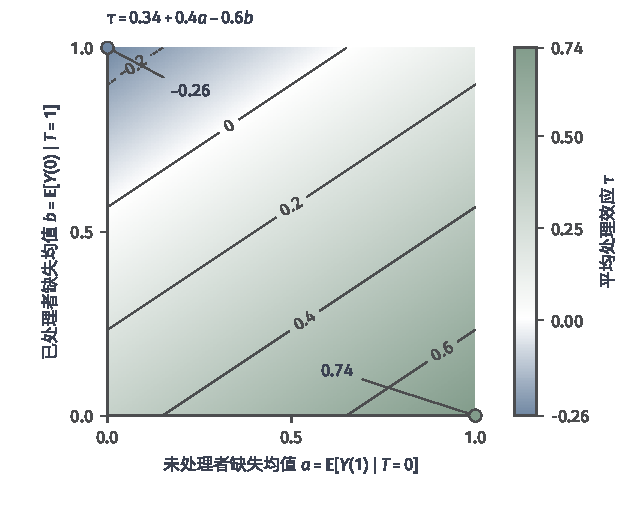
\includegraphics[width=105mm]{figures/00-shared/mathematical-preliminaries-lower/01-random-variables-distributions-and-causality/matplotlib/causal-manski-missing-outcome-geometry/figure.pdf}
  \caption{两个缺失潜在结果均值生成的Manski锐界。固定\(P(T=1)=0.6\)、已处理组观察均值\(0.7\)、未处理组观察均值\(0.2\)，并且只要求一致性及\(0\leq Y(t)\leq1\)。横、纵轴为两类缺失均值\(a,b\)，方形内全部赋值均与这些观测相容；色阶和等高线表示\(\tau=0.34+0.4a-0.6b\)。两个角点达到\(-0.26\)与\(0.74\)，范围宽度为\(1\)。色阶反映相容机制的目标差异，不是抽样误差。}
  \label{fig:causal-manski-missing-outcome-geometry}
\end{figure}

\subsubsection{支持缺口下的效应与策略界}
\label{sec:causal-support-policy-bounds}

现在假设条件交换性可信，但双侧重叠只在协变量区域\(\mathcal O\)成立。用
\(\mathcal N\)表示目标总体中缺少某种处理的区域，两者不交且覆盖目标总体。
结果仍在\([0,1]\)时，条件效应\(\tau(x)\in[-1,1]\)，故
\[
  \tau=
  \mathbb E[\tau(X)\mathbb I\{X\in\mathcal O\}]
  +\mathbb E[\tau(X)\mathbb I\{X\in\mathcal N\}].
\]
第一项由调整式识别，第二项只能先按范围控制，得到
\begin{equation}
  \begin{aligned}
    &\mathbb E[\tau(X)\mathbb I\{X\in\mathcal O\}]
      -\mathbb P(X\in\mathcal N)\leq\tau\\
    &\qquad\leq
      \mathbb E[\tau(X)\mathbb I\{X\in\mathcal O\}]
      +\mathbb P(X\in\mathcal N).
  \end{aligned}
  \label{eq:causal-overlap-gap-bounds}
\end{equation}
这是一组有效界，未声称总是锐界；缺口区域中若仍观察到一种处理的结果，
利用这一侧均值还可能收紧。限制目标人群到\(\mathcal O\)可以点识别重叠人群效应，
但已经改变了目标总体。假设缺口内效应与邻近区域平滑、同号或落在更小范围，也能
收紧答案，却都是额外外推条件，不能由已覆盖部分的拟合优度证明。

单步策略评价需要的支持可以更少。沿用式~\eqref{eq:causal-policy-value}的有限
动作集合及目标策略\(\pi\)，其中\(a\)仍表示将同一个\(T\)设为值\(a\)的行动。
记录自然处理选择的资料称为日志，记其中的动作概率为
\(e_a(x)=\mathbb P(T=a\mid X=x)\)。假设对所有动作，
\(L\leq Y(a)\leq H\)，且一致性和给定\(X\)的交换性成立。若目标覆盖条件为
\[
  \pi(a\mid x)>0\quad\Longrightarrow\quad e_a(x)>0
\]
并在目标总体中几乎处处成立，则
\[
  \begin{aligned}
    \mathbb E\left[\frac{\pi(T\mid X)}{e_T(X)}Y\middle|X\right]
    &=
    \sum_{\substack{a\in\mathcal A\\e_a(X)>0}}
      e_a(X)\frac{\pi(a\mid X)}{e_a(X)}
      \mathbb E[Y\mid T=a,X]\\
    &=
    \sum_{a\in\mathcal A}\pi(a\mid X)\mathbb E[Y(a)\mid X].
  \end{aligned}
\]
对\(X\)取期望，得到
\begin{equation}
  V(\pi)=\mathbb E\left[\frac{\pi(T\mid X)}{e_T(X)}Y\right].
  \label{eq:causal-policy-value-weighting}
\end{equation}
这是换测度（用密度比把一个分布下的期望改写为另一个分布下的加权期望）的一个因果用途：改变动作分配，
保留给定背景与动作的结果机制。权重只在日志实际可能选择的动作上求值，
覆盖条件使其余动作的目标概率为零，无须引入\(0/0\)约定。

覆盖失败时，记目标策略落入缺口的概率质量及已识别贡献为
\[
  \begin{aligned}
    r&=\mathbb E_X\left[\sum_{a:e_a(X)=0}\pi(a\mid X)\right],\\
    K&=\mathbb E_X\left[
      \sum_{a:e_a(X)>0}\pi(a\mid X)\mathbb E[Y\mid T=a,X]
    \right].
  \end{aligned}
\]
缺口部分的贡献在\([Lr,Hr]\)内，因而
\begin{equation}
  K+Lr\leq V(\pi)\leq K+Hr.
  \label{eq:causal-policy-value-bounds}
\end{equation}
两个策略的价值范围若完全分离，就能确定排序；若重叠，单独看边际范围未必能
判断。它们使用同一组未知潜在结果，不能把各自端点当作独立可选。
例如两策略完全相同时，无论各自的价值范围多宽，价值差都严格为零。
一般应对
\[
  V(\pi_1)-V(\pi_2)
  =
  \mathbb E_X\sum_a
    \bigl(\pi_1(a\mid X)-\pi_2(a\mid X)\bigr)\mathbb E[Y(a)\mid X]
\]
直接构造联合识别集合或上下界。拟合器对缺口给出的单一外推，不是额外的排序证据。

图~\ref{fig:causal-confounding-coverage}把混杂与覆盖分别数值化。左图回顾前面的
风险分层例子；右图另设结果范围为\([0,1]\)，已覆盖部分条件平均收益为\(0.6\)，
故\(K=0.6(1-r)\)。在\(r=0.2\)时，价值范围为\([0.48,0.68]\)。
宽度\(0.2\)来自缺口中的未知结果机制，不会因增加同一覆盖区域内的样本而消失。
\begin{figure*}[htbp]
  \centering
  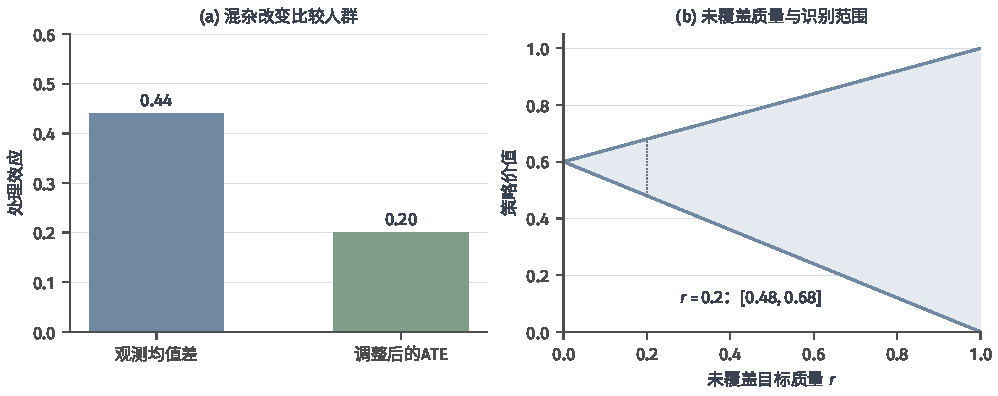
\includegraphics[width=\linewidth]{figures/00-shared/mathematical-preliminaries-lower/01-random-variables-distributions-and-causality/matplotlib/causal-confounding-coverage/figure.pdf}
  \caption{两个独立的教学构造。左图比较风险分层例子的观测均值差\(0.44\)与调整
  效应\(0.20\)。右图按式~\eqref{eq:causal-policy-value-bounds}绘制
  \([0.6(1-r),0.6(1-r)+r]\)。阴影为总体识别范围，不是抽样置信带；
  两个面板不表示同一数据集。}
  \label{fig:causal-confounding-coverage}
\end{figure*}

这里的策略只作一次行动。\BookSectionRef{sec:decision-dynamic-programming}{第~\ref{sec:decision-dynamic-programming}节}建立序贯
策略后，必须逐时检查历史覆盖、时间变化的混杂及轨迹结果定义，不能把单步权重
直接套到整条轨迹。

\subsubsection{未观测混杂下的敏感性范围}
\label{sec:causal-sensitivity-ranges}

另一种缺口不是某类记录完全没有，而是相同已观测背景下仍存在未观测选择差异。
敏感性分析不强行断言该差异为零，而是规定其允许强度，检查结论随强度怎样变化。

先用一个最小线性模型定位偏差。设变量中心化，
\[
  T=\alpha U+\varepsilon_T,\qquad
  Y=\beta T+\gamma U+\varepsilon_Y,
\]
其中\(U,\varepsilon_T,\varepsilon_Y\)两两独立、方差有限，且
\(\operatorname{Var}(T)>0\)。理想设定\(T=t\)时，固定背景的结果对\(t\)的
导数为\(\beta\)。但只将\(Y\)对自然处理\(T\)作总体线性回归，得到
\begin{equation}
  \begin{aligned}
    \beta_{\mathrm{obs}}
    &=\frac{\operatorname{Cov}(T,Y)}{\operatorname{Var}(T)}\\
    &=\beta+
      \gamma\frac{\alpha\operatorname{Var}(U)}{\operatorname{Var}(T)}.
  \end{aligned}
  \label{eq:causal-linear-confounding-bias}
\end{equation}
这里用到了
\(\operatorname{Cov}(T,Y)=\beta\operatorname{Var}(T)
+\gamma\operatorname{Cov}(T,U)\)，以及
\(\operatorname{Cov}(T,U)=\alpha\operatorname{Var}(U)\)。
共同背景同时进入处理与结果，产生了第二项。这里的\(\beta_{\mathrm{obs}}\)最小化总体均方线性预测误差，是一个常数；条件均值\(t\mapsto\mathbb E[Y\mid T=t]\)则未必为直线。
例如取\(\alpha=\gamma=1,\beta=0\)，令\(U\)等概率取\(\pm1\)、\(\varepsilon_T\sim\mathcal N(0,1)\)与\(U\)独立，且\(\varepsilon_Y=0\)。此时\(Y=U\)，两种背景的条件概率比为\(e^{2t}\)，故
\[
 \mathbb E[Y\mid T=t]=\tanh t,\qquad
 \left.\frac{\mathrm d}{\mathrm dt}\mathbb E[Y\mid T=t]\right|_{t=0}=1,
 \qquad\beta_{\mathrm{obs}}=\frac12.
\]
因此线性投影偏差不能不加条件地当作每个剂量点的导数偏差。若只知道线性投影偏差\(\beta_{\mathrm{obs}}-\beta\)的绝对值不超过
\(\Lambda\)，则
\(\beta\in[\beta_{\mathrm{obs}}-\Lambda,\beta_{\mathrm{obs}}+\Lambda]\)。
观测可以估计\(\beta_{\mathrm{obs}}\)，却不能在没有额外信息时把
\(\alpha,\gamma,\beta\)各自分开；改变函数形式也会改变敏感性参数的含义。

异质或非线性响应不一定有一个统一斜率修正量。仍记
\(\mu_t(x)=\mathbb E[Y\mid T=t,X=x]\)和\(e(x)=\mathbb P(T=1\mid X=x)\)。
在\(0<e(x)<1\)且相关条件期望有限时，定义选择偏差函数
\[
  \begin{aligned}
    b_1(x)&=\mathbb E[Y(1)\mid T=1,X=x]
            -\mathbb E[Y(1)\mid T=0,X=x],\\
    b_0(x)&=\mathbb E[Y(0)\mid T=1,X=x]
            -\mathbb E[Y(0)\mid T=0,X=x].
  \end{aligned}
\]
条件交换性蕴含\(b_1=b_0=0\)，但反过来只得到条件均值交换性，
不能推出完整潜在结果分布相同。比如两组都均值为零，一组恒等于零，另一组等概率
取\(1,-1\)，均值相同仍保留分布差异。

一致性给出
\(\mathbb E[Y(1)\mid T=1,X=x]=\mu_1(x)\)，再由全期望
\[
  \begin{aligned}
    \mathbb E[Y(1)\mid X=x]
    &=e(x)\mu_1(x)+(1-e(x))(\mu_1(x)-b_1(x))\\
    &=\mu_1(x)-(1-e(x))b_1(x).
  \end{aligned}
\]
另一侧有
\[
  \begin{aligned}
    \mathbb E[Y(0)\mid X=x]
    &=(1-e(x))\mu_0(x)+e(x)(\mu_0(x)+b_0(x))\\
    &=\mu_0(x)+e(x)b_0(x).
  \end{aligned}
\]
相减得到
\begin{equation}
  \tau(x)=\mu_1(x)-\mu_0(x)
  -(1-e(x))b_1(x)-e(x)b_0(x).
  \label{eq:causal-selection-bias-function}
\end{equation}
若领域知识仅支持
\(|b_1(x)|\leq\Gamma_1(x)\)及\(|b_0(x)|\leq\Gamma_0(x)\)，三角不等式给出
\begin{equation}
  \begin{aligned}
    \mu_1(x)-\mu_0(x)-\Delta(x)
    &\leq\tau(x)\\
    &\leq\mu_1(x)-\mu_0(x)+\Delta(x),
  \end{aligned}
  \label{eq:causal-sensitivity-bounds}
\end{equation}
其中\(\Delta(x)=(1-e(x))\Gamma_1(x)+e(x)\Gamma_0(x)\)。
重叠在目标总体几乎处处成立、潜在结果及相应控制量可积时，再对\(X\)平均便得到
ATE范围。该范围是当前偏差约束的有效包络；若还有限定结果范围或其他联合约束，
不能未经可达性检查就宣称它为锐界。

代入数值可以看清偏差约束如何影响结论。以下均值、效应与偏差均使用\(Y\)的同一
计量单位，沿用本小节的一般实值结果设定。取某个协变量分层上
\(e(x)=0.3\)、\(\mu_1(x)-\mu_0(x)=0.5\)，
并设偏差仅满足\(\Gamma_1(x)=0.2\)、\(\Gamma_0(x)=0.1\)，则
\(\Delta(x)=0.7\times0.2+0.3\times0.1=0.17\)，效应区间为
\([0.33,0.67]\)。两项的权重并不相同：\(b_1\)以\(1-e(x)\)加权，\(b_0\)以
\(e(x)\)加权。前一项修正未处理者缺失的\(Y(1)\)，后一项修正已处理者缺失的
\(Y(0)\)；若其他量固定而\(e(x)\)增大，前一项的权重减小，后一项的权重增大。

先保持\(e(x)=0.3\)及观测均值差\(0.5\)不变，只把两个偏差上界都放宽到
\(0.5\)个结果单位。此时\(\Delta(x)=0.7\times0.5+0.3\times0.5=0.5\)，效应
包络为\([0,1]\)，已经包含零；当前偏差约束不足以确定效应严格为正。这是效应的
包络，并未另外假定结果\(Y\)只能取\([0,1]\)中的值。

再恢复最初的\(\Gamma_1(x)=0.2\)、\(\Gamma_0(x)=0.1\)，保持观测均值差
\(0.5\)，仅把\(e(x)\)从\(0.3\)改为\(0.8\)，便有
\[
  \Delta(x)=0.2\times0.2+0.8\times0.1=0.12,
  \qquad \tau(x)\in[0.38,0.62].
\]
这里更大的权重移向了较小的\(\Gamma_0\)，所以包络比最初的\([0.33,0.67]\)窄；
处理比例更极端本身并不保证包络缩小，若两个上界都仍为\(0.5\)，则
\(\Delta(x)\)仍是\(0.5\)。这些比较把结论与所许偏差的门槛联系起来：本例观测
差为正，要使效应下界严格大于零，需有\(\Delta(x)<0.5\)。

为了连续比较同一类偏差假设，可固定\(e(x)=0.3\)和观测均值差\(0.5\)，令
\(\Gamma_1(x)=0.2s\)、\(\Gamma_0(x)=0.1s\)，其中\(s\geq0\)是共同放宽倍数。
于是\(\Delta(x)=0.17s\)，图~\ref{fig:causal-sensitivity-effect-envelope}中的下界在
\(s=0.5/0.17=50/17\)处恰好达到零。图中带状范围表达未观测偏差假设允许的效应包络，
不是由重复抽样得到的置信带；\(s\)也不是样本量。

\begin{figure}[htbp]
  \centering
  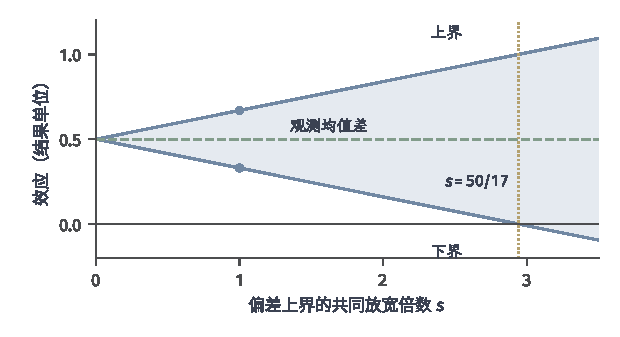
\includegraphics[width=105mm]{figures/00-shared/mathematical-preliminaries-lower/01-random-variables-distributions-and-causality/matplotlib/causal-sensitivity-effect-envelope/figure.pdf}
  \caption{选择偏差上界放宽时的效应包络。固定一个协变量分层及\(e(x)=0.3\)、\(\mu_1(x)-\mu_0(x)=0.5\)，令\(\Gamma_1=0.2s\)、\(\Gamma_0=0.1s\)。蓝线与浅蓝区域为\([0.5-0.17s,0.5+0.17s]\)，绿虚线为固定的观测均值差；\(s=1\)的两个点标出\([0.33,0.67]\)，黄竖线标出下界达到零的门槛。所有纵轴量使用相同结果单位，图中未另外约束结果只能取\([0,1]\)。}
  \label{fig:causal-sensitivity-effect-envelope}
\end{figure}

\(\Gamma_t\)是关于未观测差异的假设，不是样本自动生成的误差条。报告应展示在多大
强度下结论变号或越过决策阈值，而不只给一个恰好保留原结论的值。
其他有根据的假设也能缩小相容类。例如个体\term{单调性}（monotonicity）
\[
  Y(1)\geq Y(0)\quad\text{几乎必然}
\]
排除所有受损个体，故在加入单调性后的相容类非空时，ATE至少为零。
若已有有效范围\([L_{\mathrm{old}},U_{\mathrm{old}}]\)，应将它与\([0,+\infty)\)相交，
得到\([\max\{L_{\mathrm{old}},0\},U_{\mathrm{old}}]\)，而不是把正的已有下界降为零。
交集为空意味着单调性与当前观测或已有假设冲突，不能把空范围当成效应结论。
它比“平均有益”更强。若已知个体效应位于\([-\rho,\rho]\)，支持缺口中的
\([-1,1]\)可换成更窄范围；平滑外推也必须作为新增机制限制声明。

跨环境资料可以提供另一种约束。若源环境有随机试验，目标环境给出协变量分布，
并假设条件效应在两环境相同，且目标协变量分布对源环境分布绝对连续，即源环境
的零概率背景集在目标环境中也为零概率。再假设目标环境的两种潜在结果可积，
则相同的条件效应在目标协变量分布下也可积，并有
\[
  \tau_{\mathrm{target}}
  =\int\tau_{\mathrm{source}}(x)\,P_{X,\mathrm{target}}(\mathrm dx).
\]
这是条件效应稳定和目标覆盖共同给出的运输关系；在离散情形，覆盖要求目标中
出现的背景在源环境也有正概率。连续情形仅有拓扑支持包含还不够，应使用上述
绝对连续条件。条件效应稳定与目标覆盖条件都不能由稳定预测关联自动推出。
共同隐藏原因、选择过程或多个机制同步变化都可能产生稳定关联。

相容类也可用于第~\ref{sec:causal-counterfactual-recourse}节的反事实、补救与公平
目标。跨世界配对不同的模型可能同样解释试验边缘，却改变行动成功概率或公平判断。
此时应传播这些模型差异，而不是仅报告选定生成模型内的模拟精度。

\subsection{有限样本下的响应估计}
\label{sec:causal-response-estimation}

即使识别式成立，条件响应、处理概率与总体权重通常仍需从样本估计。比如调整法用
\(\widehat\mu_t\)代替\(\mu_t\)，再在目标背景样本上平均：
\[
  \widehat\tau
  =\frac1n\sum_{i=1}^n
    \bigl(\widehat\mu_1(X_i)-\widehat\mu_0(X_i)\bigr).
\]
这只是识别式的一种代入估计，不自动具有无偏性或某种收敛速度。拟合误差、目标样本
的抽样误差以及重复使用同一数据引入的依赖，仍须按第~\ref{sec:rv-inference}节
的估计与数据复用规则分析。采用样本拆分或交叉拟合时，应明确哪些样本拟合、哪些
样本评价，以及相应误差条件。

逆概率法还要估计倾向概率。很小但非零的真实概率允许总体识别，却可能使估计方差
很大；截断权重可改变偏差与方差，但不能被解释为凭空补足支持。更灵活的拟合器
或交叉拟合同样不能修复交换性错误。

部分识别时，估计对象可以是识别集合的端点或其外包络。识别集合在总体分布已知时
仍可能不是单点，表达机制歧义；\term{置信区间}来自有限样本，表达总体目标、
识别集合或端点的估计误差。对端点构造置信范围，还需按所用统计方法处理两个端点
共同的覆盖要求，不能把端点估计直接当作已知真界。

实际报告应分别列出相容机制留下的范围、抽样造成的不确定性，以及积分或优化中的
数值误差。增加样本主要改善第二项，改善算法主要影响第三项；改变设计、扩大目标
行动覆盖或加入可辩护的机制限制，才可能缩小第一项。尤其在效应符号或行动阈值附近，
应同时报告对支持处理、敏感性参数及目标总体选择的依赖。

\section{因果生成结构的表示}
\label{sec:causal-generating-structure}

培训可以先改变技能，技能再改变成绩，这类“一步步如何产生”的过程很难只用一个整体映射看清。更自然的写法是为每个变量单独给出一条局部生成规则：培训由个人情况决定，技能由培训和天赋决定，成绩由培训、技能和其他因素决定。把这些局部规则合起来，就能构造此前使用的整体响应映射。每条局部方程规定怎样产生一个变量，背景的联合分布规定未展开因素怎样共同变化，图则记录方程读取哪些变量。只有把这三项结合，才能计算替换处理规则后应沿哪些关系重新求值。

\subsection{局部机制的结构方程表示}
\label{sec:causal-local-structural-equations}

把模型内需要解释的变量称为内生变量，把当前模型不再解释的背景称为外生变量。
“外生”是相对于模型边界而言，并不意味着这些量在现实中没有原因，也不自动意味着
它们彼此独立。进入某个变量生成函数的其他内生变量称为它的父变量，表示该局部机制
直接读取哪些输入。

这些局部方程为什么要求“无环”？因为我们希望给定背景后，每个变量都能被一步步算出来，而不是陷入“甲依赖乙、乙又依赖甲”的循环。有环时方程可能无解或有无穷多解（本章末会给出例子），干预之后也无法确定该按什么次序重新求值。无环结构保证存在一个求值次序，使每个变量被计算时它所依赖的变量都已经算好。
\begin{definition}[无环结构因果模型]
  \label{def:causal-structural-model}
  本章的\term{结构因果模型}（structural causal model, SCM）由内生变量
  \(\bm V=(V_1,\ldots,V_d)\)的可测状态空间、外生背景
  \(\bm U=(U_1,\ldots,U_d)\)的联合分布及可测结构函数组成：
  \begin{equation}
    V_j=f_j(\operatorname{pa}_j,U_j),
    \qquad j=1,\ldots,d.
    \label{eq:causal-scm-definition}
  \end{equation}
  其中\(\operatorname{pa}_j\)收集进入第\(j\)个函数的其他内生变量。
  \term{无环}（acyclic）要求存在节点次序\(j_1,\ldots,j_d\)，使每个函数的
  内生输入都来自次序中更早的节点。外生分量可以相关。
\end{definition}

把每个内生变量画成节点，在\(V_k\)作为输入进入\(f_j\)时画箭头\(V_k\to V_j\)，
便得到有向无环图，简称DAG。上述求值次序已足以理解无环性，不需要先学习图排序
算法。SCM的箭头具有生成语义；若箭头只用于表示联合分布的条件分解，就不能据此
判断改变输入的后果\scite{math-pearl2009causality}

例如，培训\(T\)、技能\(M\)和成绩\(Y\)可以写成
\[
  T=f_T(U_T),\qquad
  M=\alpha T+U_M,\qquad
  Y=\beta T+\gamma M+U_Y.
\]
这里的直接输入关系为\(T\to M\)、\(T\to Y\)、\(M\to Y\)。若
\(U_T,U_M,U_Y\)相关，处理选择还可能与技能或成绩背景相联系；仅画出这三条内生边
不足以表示全部共同背景。要使用独立噪声DAG的概率规则，必须另行要求这些背景独立，
或把相关性的共同来源显式放进模型。

有限维模型可以把局部函数写成\(f_{j,\bm\theta_j}\)，并用
\(\bm\theta=(\bm\theta_1,\ldots,\bm\theta_d)\)汇集参数。上例的
\(\alpha,\beta,\gamma\)是局部作用参数；一般SCM则不必属于有限维函数族。
指定关系但不知道函数，或拟合函数却没有确定它的因果语义，都仍留下结构上的未知。

\subsection{局部机制的复合与响应生成}
\label{sec:causal-mechanism-composition}

有了局部方程，定义~\ref{def:causal-response-interface}假定的自然映射就可以
实际构造。无环次序让每一步只读取已经得到的值，因此既给出计算过程，也排除了
同一背景下出现多个自然解的歧义。

\begin{theorem}[无环机制的唯一可测响应]
  \label{thm:causal-acyclic-response}
  对定义~\ref{def:causal-structural-model}中的模型，每个背景
  \(\bm u\)唯一确定一组满足所有结构方程的内生取值。
  所得自然映射\(F_M:\mathcal U\to\mathcal V\)可测。将任意指定的一组方程
  替换为常量方程后，所得映射\(F_M^a\)同样存在、唯一且可测。
  对单变量理想干预，响应\((t,\bm u)\mapsto R_M(t,\bm u)\)联合可测。
\end{theorem}
\begin{proof}
  取符合无环性的次序\(j_1,\ldots,j_d\)。第一个变量没有内生父变量，
  因而\(v_{j_1}=f_{j_1}(u_{j_1})\)唯一确定，且是\(\bm u\)的可测函数。
  假设前\(k-1\)个变量已唯一确定为可测函数。第\(k\)个方程的父变量都在其中，
  将这些函数及\(u_{j_k}\)代入可测的\(f_{j_k}\)，便得到唯一且可测的
  \(v_{j_k}\)。归纳到\(d\)，得到满足全部方程的可测向量\(F_M(\bm u)\)。
  任何另一组解在第一个坐标都必须相同；逐坐标应用同一理由，便证明唯一性。

  常量替换只删除输入，不增加逆向依赖，原次序仍可使用。被替换坐标直接取行动
  指定值，其余坐标按同样归纳求出，从而得到\(F_M^a\)。
  若把处理值\(t\)也作为输入，被替换坐标是乘积空间上的投影
  \((t,\bm u)\mapsto t\)，其余步骤仍是可测函数的复合，因此
  \(F_M^{a(t)}(\bm u)\)及其结果坐标\(R_M(t,\bm u)\)联合可测。
\end{proof}

自然分布是\((F_M)_{\#}P_{\bm U}\)，干预分布是
\((F_M^a)_{\#}P_{\bm U}\)。两个推前共用同一个背景分布，只改变生成映射。
若理想干预值恰好等于该背景下的自然处理值，那么自然解也满足替换后的全部方程；
由唯一性，两组解相同。这也证明了这种构造中的一致性，而不只是另行假定
\(Y=Y(T)\)。

若结果方程为\(Y=f_Y(T,X,U_Y)\)，且\(X\)不受处理干预影响，则
\begin{equation}
  Y(t)=f_Y(t,X,U_Y).
  \label{eq:causal-scm-potential-outcome}
\end{equation}
因此\(\mathcal L(Y(t))=\mathcal L(Y\mid\operatorname{do}(T=t))\)。
若结果还依赖处理会改变的技能\(M\)，则必须先重算\(M(t)\)，不能仍代入事实技能。
对上面的线性机制，
\[
  M(t)=\alpha t+U_M,\qquad
  Y(t)=(\beta+\gamma\alpha)t+\gamma U_M+U_Y,
\]
所以整体响应导数为\(\beta+\gamma\alpha\)，不只是局部结果方程中固定\(M\)
时的偏导数\(\beta\)。取\(\alpha=2,\beta=1,\gamma=3\)，增加一单位培训使成绩
增加\(7\)，其中直接贡献为\(1\)，经技能传递的贡献为\(6\)。
对可微的非线性机制\(M=f_M(T,U_M)\)、\(Y=f_Y(T,M,U_Y)\)，链式法则给出
\[
  \frac{\partial R_M(t,\bm u)}{\partial t}
  =
  \frac{\partial f_Y}{\partial t}
  +
  \frac{\partial f_Y}{\partial m}
  \frac{\partial f_M}{\partial t},
\]
各偏导数均在该背景的干预取值处计算。这连接了第~\ref{sec:causal-local-response}节
的整体局部变化与本节的局部方程；对它再作总体平均，仍须检查导数与积分交换条件。

图~\ref{fig:causal-direct-mediated-total-response}沿用\(\alpha=2,\beta=1,\gamma=3\)，再固定背景\(U_M=U_Y=0\)，将“保留技能方程”和“固定技能值”分开计算。只设置培训\(T=t\)时，原技能规则仍要读取新的处理值，所以\(M(t)=2t\)，总成绩为\(Y(t)=t+3(2t)=7t\)。若另加一项把技能同时固定为\(0\)的联合干预\(\operatorname{do}(T=t,M=0)\)，成绩才变成\(t\)。右图把从\(t=0\)到\(1\)的增量分成直接的\(1\)与经技能传递的\(3\times2=6\)：去掉后者改变了行动目标，不能仍把剩下的\(1\)称为只改变培训的总响应。

\begin{figure*}[htbp]
  \centering
  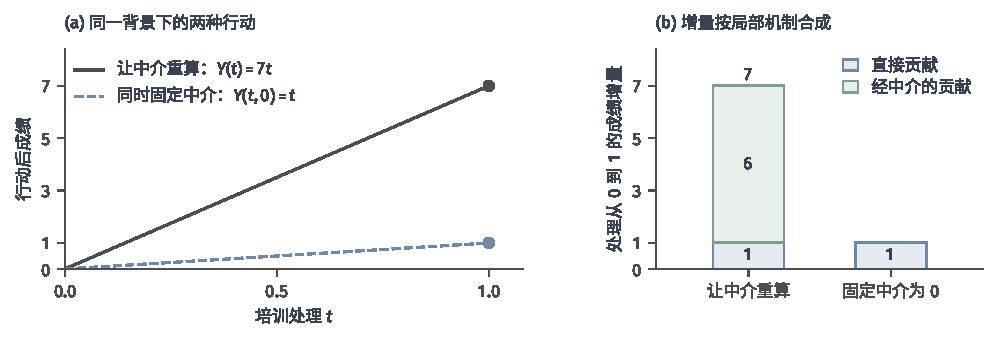
\includegraphics[width=169mm]{figures/00-shared/mathematical-preliminaries-lower/01-random-variables-distributions-and-causality/matplotlib/causal-direct-mediated-total-response/figure.pdf}
  \caption{局部规则的复合与总响应。教学机制为\(M=2T+U_M\)、\(Y=T+3M+U_Y\)，背景固定为\(U_M=U_Y=0\)。左图灰实线只设置\(T=t\)，让技能按原方程重算；蓝虚线同时设置\(T=t,M=0\)，图中以\(Y(t,0)\)表示这一联合干预结果。右图比较两种行动从\(t=0\)到\(1\)的成绩增量，蓝色为直接贡献\(1\)，绿色为经技能传递的贡献\(6\)。曲线与柱高来自同一给定线性机制，不是观测回归系数，也不建立一般中介效应的识别结论。}
  \label{fig:causal-direct-mediated-total-response}
\end{figure*}

\begin{example}[计算模型中的受控替换]
  \label{ex:causal-controlled-computation}
  一套参数已经固定的程序先计算中间读数，再把这个读数与其他输入合成输出。
  我们希望检查输出是否依赖实际读到的内容，因而把程序本身作为此次研究的生成机制，
  指定哪些计算保持原样、在哪一步替换数值。这个问题与推断程序外部的现实机制不同。

  设输入为\(\bm x\in\mathbb R^d\)，保留条件为\(\bm c\in\mathbb R^r\)，
  中间读数为\(\bm h\in\mathbb R^k\)，标量输出为\(\widehat y\)。固定参数
  \(\bm\theta\)以后，原程序为
  \[
    \bm h=f_{\bm\theta}(\bm x,\bm c),\qquad
    \widehat y=g_{\bm\theta}(\bm x,\bm h,\bm c).
  \]
  \(\bm c\)收集此次比较保留的其他输入和已有历史；这里先假定计算是确定性的。
  若程序含随机计算，还须固定两次运行所用的外生随机数，或另行声明对哪些随机量取平均。

  检查某次读取的作用时，保持\(\bm x,\bm c,\bm\theta\)不变，只在程序实际消费
  \(\bm h\)的位置把它换为同维且程序可接受的值\(\bm v\)，并沿原有规则重算所有受影响的后继量。
  替换后的输出与原输出之差为
  \begin{equation}
    \Delta_{\mathrm{read}}(\bm v;\bm x,\bm c)
    =g_{\bm\theta}(\bm x,\bm v,\bm c)
    -g_{\bm\theta}\bigl(\bm x,f_{\bm\theta}(\bm x,\bm c),\bm c\bigr).
    \label{eq:causal-computational-read-replacement}
  \end{equation}
  这就是把读数方程替换为\(\bm h=\bm v\)所产生的程序响应。若一次读取还涉及
  替换之前已经确定的条目选择、读取位置或读取权重，而目标只比较被消费的内容，这些量也须保持原样；
  同时改变它们得到的是另一项干预。

  若改的是输入记录\(\bm x\mapsto\bm x'\)，中间读数也应按原规则重新计算，得到
  \[
    \widehat y_{\mathrm{input}}(\bm x';\bm c)
    =g_{\bm\theta}\bigl(\bm x',f_{\bm\theta}(\bm x',\bm c),\bm c\bigr).
  \]
  把输入改为\(\bm x'\)却保留原读数，对应同时设置输入和读数，通常不等于这项
  输入替换。删除整个模块、改变参数或重新训练又会替换更多规则，回答的也不是同一问题。

  只要替换值在程序接受的定义域内，以上响应就能通过运行程序求出。
  替换值即使偏离训练分布，也不自动使程序响应失去定义；但这次响应不能直接概括
  训练分布内其他输入上的内容依赖，更不能单凭它推断现实中的因果效应。
  要回答现实变量改变后结果会怎样，还须说明程序输入怎样对应现实变量、行动会改变
  哪些后继因素，以及固定的计算规则是否仍能代表这些因素的生成机制。
  因而，受控替换直接支持的是指定程序、指定位置和指定替换下的输出比较；
  从这一比较到现实行动的效果，仍需本章前面讨论的机制假设与识别依据。
\end{example}

回到结构因果模型，在外生噪声相互独立时，还可以用局部概率核表达同一生成计算。记
\[
  K_j(B\mid\bm v_{\operatorname{pa}_j})
  =
  \mathbb P\bigl(f_j(\bm v_{\operatorname{pa}_j},U_j)\in B\bigr).
\]
每个核都由机制及噪声分布指定，沿无环次序复合这些核便得到联合分布。独立性保证
当前噪声不会被已经生成的变量额外筛选。若每个局部核相对于固定的坐标参考测度
\(\mu_j\)都有可测密度，联合参考测度取\(\bigotimes_j\mu_j\)，则
\[
  p(\bm v)=\prod_{j=1}^d p(v_j\mid\operatorname{pa}_j).
\]
离散坐标可取计数测度，相应密度就是质量函数。不满足这种支配条件时，
仍用概率核的复合与积分表达联合规律。
在上述受支配情形中，理想干预把处理核换成点质量，其余核保持原样，于是得到\term{截断分解}
\begin{equation}
  p(\bm v_{-T}\mid\operatorname{do}(T=t))
  =
  \prod_{j:V_j\ne T}
  p(v_j\mid\operatorname{pa}_j)\big|_{T=t}.
  \label{eq:causal-truncated-factorization}
\end{equation}
这里\(\bm v_{-T}\)表示删除处理坐标后的变量集合。公式来自机制替换，不是对
任意概率分解删除一个因子都能得到因果分布。外生噪声相关时，上述独立核复合一般
不成立；应回到完整背景的推前，或显式展开相关来源。

局部因子必须使用结构机制指定的版本。观测分布只在父变量实际出现的支持上确定
条件分布；干预若产生了未见过的父变量组合，机制可以给出答案，但资料未必能识别
该答案。随意补一个支持外的条件密度，不会把模型外推变成数据结论。

对简单结构\(X\to T\)、\(X\to Y\)、\(T\to Y\)，用独立的新随机量按
\(q(t\mid x)\)分配处理，并保持其余独立噪声机制不变。
在上述共同参考测度下，若新处理核也具有密度\(q\)，得到
\begin{equation}
  p^q(x,t,y)=p(x)q(t\mid x)p(y\mid t,x).
  \label{eq:causal-stochastic-intervention}
\end{equation}
这正是第~\ref{sec:causal-intervention-potential-outcomes}节随机干预构造的局部
表达。确定性策略用点质量核表示，不必假装它有通常的Lebesgue密度。
策略若同时改变参与人群、结果测量或其他机制，就不能只替换处理因子。
更一般的机制替换也需要保证修改后的方程有明确解；添加依赖关系时，原无环次序
可能不再适用。

循环方程说明这一边界并非形式问题。例如\(V_1=V_2+1,V_2=V_1\)无解，而
\(V_1=V_2,V_2=V_1\)有无穷多组解。反馈系统可能需要动态演化、平衡选择或额外
唯一性条件，不能直接套用本节递归证明。

\subsection{变量关系的图表示与调整条件}
\label{sec:causal-graph-adjustment}

给定结构函数以后，逐个代入就能生成干预响应。选择调整变量时却未必需要知道每个函数的具体形式：我们要判断哪些处理前背景足以阻断处理选择与结果之间的联系。图只保留局部方程的输入关系，将满足同一结构的机制放在一起考察。局部路径说明条件化为何可能消除或制造联系；全图检查再判断是否还留有其他路径，后门准则据此为前面的调整公式提供充分条件。

\subsubsection{局部因果关系与调整影响}
\label{sec:causal-local-path-patterns}

结构\(T\leftarrow X\to Y\)把\(X\)称为\(T\)与\(Y\)的
\term{共同原因}（common cause）。即使处理并不影响结果，不同\(X\)人群接受
处理的比例不同，也会使\(T,Y\)在自然记录中相关。这是混杂产生的一种方式。
第~\ref{sec:causal-adjustment-identification}节的风险分层算例正是通过在同一背景层
比较，再用同一目标权重平均，消除了由两组构成不同造成的差异。

结构\(T\to M\to Y\)中的\(M\)是\term{中介变量}（mediator）：处理对结果的
一部分影响经过它传递。若目标是总效应，固定\(M\)会阻断这部分变化；若研究同时
设定\(T=t,M=m\)的响应，则需明确这是不同的联合干预。
在线性例子中，固定中介后的处理系数为\(\beta\)，让中介随处理变化的总系数为
\(\beta+\gamma\alpha\)。这并不建立一般路径效应的识别公式，只说明两种目标不同。

结构\(T\to C\leftarrow Y\)中的\(C\)是\term{碰撞点}（collider），两条箭头
在此相遇，形象地说就是两条因果链“对撞”到同一个变量上。不以\(C\)筛选时，这条路径本身不要求两端相关；一旦给定\(C\)（按它分层、只看某个子群，或用它做选择），却可能
引入关联。这是三种结构里最反直觉的一种，值得用例子记住。例如两个独立能力共同决定总分，入选要求总分超过阈值且两项能力可以
补偿，那么入选者中一项能力较弱的人往往需要另一项更强——两项本来独立的能力，在“已入选”这个子群里变成了负相关。若入选规则改成两项能力
分别超过各自阈值，这种负关联未必出现。关系的方向取决于选择机制，不能把选择
后的相关解释为一种能力造成另一种能力。

图~\ref{fig:causal-local-path-patterns}用双边框标记已经给定的中间变量。共同原因和中介在所画路径上都是非碰撞点，给定它们会关闭该路径；给定碰撞点则会打开原本关闭的路径，但路径活跃并不保证实际分布一定存在非零统计依赖。调整变量的作用因而取决于它在路径中的角色。较大图还可能有多条连接同一对变量的路径，关闭一个局部片段后须继续检查其他路径。
\begin{figure*}[htbp]
  \centering
  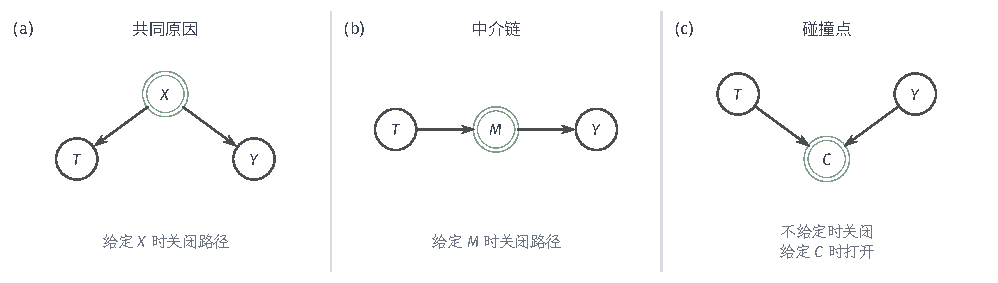
\includegraphics[width=\linewidth]{figures/00-shared/mathematical-preliminaries-lower/01-random-variables-distributions-and-causality/tikz/causal-local-path-patterns/figure.pdf}
  \caption{共同原因、中介与碰撞点的局部路径。双边框表示节点已加入条件集。
  共同原因和中介是非碰撞点，给定后关闭这条路径；给定碰撞点则打开原本关闭的
  路径。路径打开表示图不再保证相应独立性，并不指定相关的大小或正负。}
  \label{fig:causal-local-path-patterns}
\end{figure*}

\subsubsection{全图路径分离与概率约束}
\label{sec:causal-global-path-separation}

较大图中，关闭一个局部片段仍可能留下另一条联系。设
\(\mathcal G=(V,E)\)是有向无环图，\(V\)是节点集、\(E\)是有向边集。
沿一条路径检查时，条件集中的非碰撞点会阻断路径；碰撞点自身及其后代都未被给定时，
该位置也阻断路径。只有每个位置都通过检查，整条路径才活跃。若连接两组节点的每条路径
都被阻断，就得到图分离；增加条件可能打开碰撞路径，因而分离未必保持。
相关的路径、碰撞点、分离与图分解计算工具可参考
\BookChapterRef{chap:graph-paths}{卷1《数学准备：计算、分析与几何》“图”部分的“图中的路径与连接关系”章}。
本节把它们接到生成模型中的概率约束。路径指底层图中相邻且互不重复的节点序列，
有向路径才要求沿箭头前进；祖先和后代均不包括节点自身。

\begin{definition}[图分离与概率独立的记号]
  \label{def:causal-d-separation}
  对两两不交的节点集\(A,B,S\)，其中\(A,B\)非空，
  \(A\perp_{\mathcal G}B\mid S\)表示图中连接\(A,B\)的每条路径都被\(S\)
  阻断；活跃路径的碰撞与非碰撞规则沿用上文逐点检查规则。
  若各节点承载随机变量，\(X_A\perp X_B\mid X_S\)则表示给定\(X_S\)后，
  \(X_A,X_B\)的条件联合分布分解为条件边缘分布的乘积。
  前一个记号只依赖图，后一个记号依赖概率分布；二者之间的联系需要模型假设。
\end{definition}

碰撞点是相对于某一条路径而言的，同一节点在不同路径上可以扮演不同角色。
给定其后代也可能传回选择信息，因此不能只检查碰撞点本身是否在条件集。
以同时含有
\[
  X\to M\to Y,\qquad X\to C\leftarrow Y,\qquad C\to D
\]
的图为例，\(X,Y\)之间有经过\(M\)和经过\(C\)的两条路径。四种条件集给出
不同判断：
\begin{itemize}
  \item \(S=\varnothing\)：经过\(M\)的链活跃，经过\(C\)的碰撞路径关闭，
  因而两端仍然d-连接。
  \item \(S=\{M\}\)：链被关闭，碰撞路径也仍关闭，所以
  \(X\perp_{\mathcal G}Y\mid M\)。
  \item \(S=\{M,C\}\)：链仍关闭，但给定碰撞点打开下方路径，两端重新d-连接。
  \item \(S=\{M,D\}\)：给定碰撞点的后代也打开下方路径，两端同样d-连接。
\end{itemize}
图~\ref{fig:causal-d-separation-paths}显示第二种情形。这个例子在本章即可逐路
检查；一般图仍须按上文规则枚举全部相关路径，不能只检查图中最显眼的一条。
\begin{figure}[htbp]
  \centering
  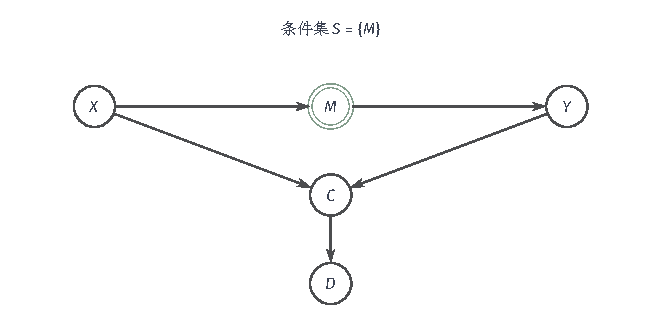
\includegraphics[width=\linewidth]{figures/00-shared/mathematical-preliminaries-lower/01-random-variables-distributions-and-causality/tikz/causal-d-separation-paths/figure.pdf}
  \caption{多条路径下的d-分离。双边框节点\(M\)属于条件集，上方链式路径关闭；
  碰撞点\(C\)及其后代\(D\)都未给定，下方路径也关闭。若再把\(C\)或\(D\)
  加入条件集，下方路径就会打开，说明增加条件可能破坏原有的分离。}
  \label{fig:causal-d-separation-paths}
\end{figure}
\FloatBarrier

图中的阻断只是关于路径的组合判断，尚未自动给出模型分布中的条件独立。若要用图选择调整变量，就需要把这两层接起来：图上已经分离的变量，在模型分布中也应条件独立。下面明确这项由图到概率的要求；随后说明独立外生背景的无环生成模型为何支持它。
\begin{definition}[因果Markov性]
  \label{def:causal-markov-property}
  分布\(P\)相对于因果DAG \(\mathcal G\)满足\term{因果Markov性}
  （causal Markov property），是指对任意两两不交的节点集\(A,B,S\)，
  \[
    A\perp_{\mathcal G}B\mid S
    \quad\Longrightarrow\quad
    \bm V_A\perp\bm V_B\mid\bm V_S.
  \]
  其中\(\bm V_A,\bm V_B,\bm V_S\)分别收集对应节点的随机变量。
\end{definition}

左边是图规则，右边是分布性质。因果Markov性把前者的阻断结论转成条件独立；
它没有说d-连接一定产生统计依赖，也没有从观测独立直接反推箭头。它与时序过程
“给定当前状态后无须更早历史”的Markov性质使用不同对象和条件集，不能只因名称
相同就互相代入。

对DAG，这一全局表述等价于局部表述：每个变量在给定父变量后，与其非后代中除
自身和父变量外的变量条件独立。独立外生噪声的无环SCM满足这一性质。
直观上，非后代及父变量不读取当前节点的独立噪声；给定父变量后，当前变量剩下
的随机性就来自这一噪声。对局部核乘积，按逆向求值次序逐个积分掉无关后代，
每次被消去的条件核积分为一，由此保留所需的局部条件因子。分解与d-分离的
全局对应是DAG的标准结论\scite{math-pearl2009causality}
把图分离转成概率独立，
还需要这里的DAG分解或生成机制条件，不能只凭连接结构推出。
若背景相关而共同来源没有入图，不能仍对这个省略后的DAG直接宣称因果Markov性。

\subsubsection{后门条件下的调整变量选择}
\label{sec:causal-backdoor-selection}

第~\ref{sec:causal-adjustment-identification}节直接假定条件交换性，再证明调整
识别。若已给出具有生成语义的因果图，就可以进一步从路径判断哪些变量可用于调整。这里要保留处理到结果的有向因果作用，并阻断后门准则指定的非因果联系；“有向因果路径”与“后门路径”并不穷尽图上两点间的所有路径。例如\(T\to C\leftarrow U\to Y\)既不是从\(T\)到\(Y\)的有向路径，也不是以箭头进入\(T\)的后门路径；其中碰撞点\(C\)在未被条件化时就阻断了这条路径。因而应先明确路径与阻断的定义，再使用下面的充分准则，不把所有非因果路径都称作后门，也不将有向因果路径另称为前门识别。
从\(T\)到\(Y\)且第一条边指向\(T\)的路径称为
\term{后门路径}（back-door path），它从处理的自然生成来源进入比较，而非沿
处理对结果的有向作用出发。

\begin{definition}[单处理、单结果的后门准则]
  \label{def:causal-backdoor-criterion}
  设\(T,Y\)是因果DAG中的不同节点，\(Z\)与\(\{T,Y\}\)不交。若\(Z\)
  不含\(T\)的后代，且给定\(Z\)阻断所有从\(T\)到\(Y\)、第一条边指向
  \(T\)的路径，则称\(Z\)满足相对于\((T,Y)\)的
  \term{后门准则}（back-door criterion）。
\end{definition}

阻断按定义~\ref{def:causal-d-separation}判断，把碰撞点放进\(Z\)可能打开
原本关闭的路径。最基本的代表图为\(Z\to T,Z\to Y,T\to Y\)，独立噪声机制给出
\[
  p(z,t,y)=p(z)p(t\mid z)p(y\mid t,z).
\]
将处理机制替换为常量\(t\)后，
\(p(z,y\mid\operatorname{do}(T=t))=p(z)p(y\mid t,z)\)。再对背景积分，得到
\begin{equation}
  p(y\mid\operatorname{do}(T=t))
  =
  \int p(y\mid t,z)p(z)\,\mathrm dz.
  \label{eq:causal-backdoor-adjustment}
\end{equation}
离散背景用求和，一般空间用对\(P_Z\)的核积分。对结果再取期望，就回到
式~\eqref{eq:causal-g-formula}的调整表示。

一般后门准则在独立噪声无环SCM、图正确包含相关共同原因且干预保留其他机制的
条件下，给出同样的调整结论\scite{math-pearl2009causality}
阻断全部后门路径排除了自然处理选择沿这些路径携带的背景差异，非后代条件保证
用于平均的\(Z\)不先被行动改变。这些是生成结构对交换性的充分支持，而不是只由
一个观测分布满足Markov性就能推出的干预结论。即使图条件成立，要从观测资料
确定积分中的局部响应，还需要目标总体内所用处理的支持条件；图不会填补空白
协变量--处理组合。

三个局部图可以核对变量角色。在\(T\leftarrow X\to Y\)中，\(X\)关闭后门；
在\(T\to M\to Y\)中，\(M\)是后代，固定它会改变总效应目标；
在\(T\to C\leftarrow Y\)中，空条件集已经关闭碰撞路径，加入\(C\)反而打开它。
因此，处理前测量、与结果相关或能提高预测精度，都不是充分的调整标准。

下面用三个小算例分别核对这些角色。先在\(T\to C\leftarrow Y\)中取\(T\)与
\(Y\)独立，各以概率\(1/2\)取\(0\)或\(1\)，并令\(C=T\oplus Y\)（两者
相同时为\(0\)，不同时为\(1\)）。无条件时\(\mathbb P(T=1\mid Y=1)=1/2\)，
两者没有关联；但在\(C=1\)子群中，\(\mathbb P(T=1\mid Y=1,C=1)=0\)。
这是因为筛选只留下\((T,Y)=(0,1),(1,0)\)两类记录，原本独立的变量在这个
子群内成为完全负相关。

子群关联还应与按全部\(C\)层标准化的总体量区分。记层内均值差为
\(\delta_c=\mathbb E[Y\mid T=1,C=c]-\mathbb E[Y\mid T=0,C=c]\)。
在\(C=0\)层有\(Y=T\)，在\(C=1\)层有\(Y=1-T\)，因此
\[
  \delta_0=1-0=1,\qquad \delta_1=0-1=-1.
\]
两层的概率各为\(1/2\)，所以若仿照调整式对它们平均，得到
\[
  \sum_{c\in\{0,1\}}\mathbb P(C=c)\delta_c
  =\frac12\times1+\frac12\times(-1)=0.
\]
这个模型中改变\(T\)只改变\(C\)，不改变\(Y\)的规则，真实总效应也是零。
该算例说明的是在\(C=1\)子群中筛选会制造关联，没有展示总体调整后的偏差或
效应符号反转。这里的正负相消也不能用来保证一般模型中按碰撞点调整仍然有效；
图上路径一旦打开，原来的独立性保证就已失去。

再看中介图\(T\to M\to Y\)。令\(T\sim\operatorname{Bernoulli}(1/2)\)，
噪声\(\eta,\varepsilon\)均为标准正态，且\(T,\eta,\varepsilon\)相互独立，
机制为\(M=T+\eta\)、\(Y=M+\varepsilon\)。设置\(T=t\)后，中介随处理重新
生成，故
\[
  Y(t)=t+\eta+\varepsilon,\qquad
  \mathbb E[Y(t)]=t,\qquad \tau=1.
\]
若改为按观测中介\(M=m\)分层，则由\(\varepsilon\)独立于\((T,M)\)且均值
为零，得到
\[
  \mathbb E[Y\mid T=t,M=m]
  =m+\mathbb E[\varepsilon\mid T=t,M=m]=m.
\]
这里使用该连续密度模型给出的条件均值版本。给定任一处理，\(M\)的正态密度在
每个实数\(m\)处均为正，因此两种处理在这些中介取值附近都有记录；不要求精确
事件\(\{M=m\}\)本身有正概率。层内两组均值差为\(m-m=0\)，而总效应为\(1\)：
固定中介没有保留处理经中介传递的作用。

“按观测\(M\)分层”与“主动同时设定\(T,M\)”仍是不同操作。若研究的是联合干预
\(\operatorname{do}(T=t,M=m)\)，本例得到\(Y=m+\varepsilon\)，故固定同一
\(m\)时的受控处理效应也为零。这个数值一致依赖当前机制与独立噪声，不能据此
把观测条件化和联合干预一般地等同。估计总效应时，要让中介按各处理下的规律变化。

最后在纯共同原因图\(T\leftarrow X\to Y\)中，明确给出二元处理的分配机制。
令\(X\sim\operatorname{Bernoulli}(1/2)\)、\(W\sim\operatorname{Unif}(0,1)\)
和标准正态噪声\(\zeta\)相互独立，并设
\[
  T=\mathbf 1\{W\leq0.2+0.6X\},\qquad Y=2X+\zeta.
\]
于是\(e(0)=0.2,e(1)=0.8\)，每个\(X\)层内的两种处理都有正概率。
Bayes公式给出\(\mathbb P(X=1\mid T=1)=0.8\)、
\(\mathbb P(X=1\mid T=0)=0.2\)，故
\[
  \begin{aligned}
    \mathbb E[Y\mid T=1]&=2\times0.8=1.6,\\
    \mathbb E[Y\mid T=0]&=2\times0.2=0.4.
  \end{aligned}
\]
观测差为\(1.2\)，来自两组\(X\)构成的差异。按\(X\)分层则有
\(\mathbb E[Y\mid T=t,X=x]=2x\)，所以每层均值差为零，调整后为
\[
  \sum_{x\in\{0,1\}}\mathbb P(X=x)(2x-2x)=0.
\]
直接核对干预也得到同一答案：替换处理规则不改变\(X\)和\(Y\)的机制，
\(Y(t)=2X+\zeta\)的均值恒为\(1\)，因而真实总效应为零。这个完整构造才允许
把观测差归于共同原因；仅有两组均值不同并不足以作这种归因。

在上述特定图中估计总效应，共同原因\(X\)可用于层内比较并按同一总体权重平均；
中介\(M\)应随处理重新生成，以保留间接作用；按碰撞点\(C\)筛选可能制造关联。
一般情况下，调整集合的选择仍取决于完整因果图、所求总效应或直接效应，以及
所用识别方法，必须检查全部相关路径和处理支持，不能只按变量名称决定。
后门准则是充分条件，不是识别的必要条件；它不适用时，随机设计、其他识别规则
或更具体的机制假设仍可能确定所选目标。

\section{因果生成结构的推断}
\label{sec:causal-structure-discovery}

给定图与局部机制，可以从背景逐步生成结果。反过来，仅看到结果记录时，需要辨认两类未知：一是变量之间的关系结构——谁是因、谁是果，哪些变量进入同一条方程；二是在结构已经给定时，每条局部方程的具体形式、参数和噪声规律。关系推断改变候选图，机制推断改变给定图上的函数和噪声；两项都会影响最终算出的响应。需要强调的是，把联合分布拟合得再好，通常也只能说明候选模型与观测相容，并不能唯一确定箭头方向或同一个体的反事实，这些还需要干预、环境变化或额外结构假设。

\subsection{变量关系的推断}
\label{sec:causal-relation-inference}

从图推出分布约束与从分布反推图，是方向相反的两项任务。要用条件独立排除候选
关系，需要说明哪些独立是真正的结构阻断，哪些可能来自参数抵消。还要说明记录
来自同一观测环境、受控干预还是不同环境，因为这些资料对候选机制提供的限制不一样。

\subsubsection{观测资料下的关系识别}
\label{sec:causal-observational-structure}

前面在生成假设下从图上分离推出分布中的条件独立。结构推断需要反向使用这些约束：给定可观测分布时，检查哪些候选图与它的条件独立关系相容；只有有限观测记录时，则还需估计和检验这些关系，不能把未检出依赖直接当成精确独立。反向使用独立约束还须排除参数抵消等巧合，即图上没有分离的变量却在相应条件分布中独立。下面的忠实性假设要求这些分布独立关系都能由图结构解释，而不是由特定参数抵消产生。
\begin{definition}[相对于DAG的忠实性]
  \label{def:causal-faithfulness}
  分布\(P\)相对于DAG \(\mathcal G\)满足\term{忠实性}（faithfulness），若对
  任意两两不交的节点集\(A,B,S\)，
  \[
    \bm V_A\perp\bm V_B\mid\bm V_S
    \quad\Longrightarrow\quad
    A\perp_{\mathcal G}B\mid S.
  \]
\end{definition}
忠实性要求分布中出现的条件独立能由图结构解释，不是由特殊参数抵消、确定性
约束或未处理的误差相关造成。因果Markov性给出正向蕴含，忠实性补上反向蕴含，
两者不能互相替代。

例如，设\(X,U_M,U_Y\)相互独立，
\(M=\alpha X+U_M\)，\(Y=\beta X+\gamma M+U_Y\)。
当\(\alpha,\gamma\ne0\)且\(\beta=-\gamma\alpha\)时，
\(Y=\gamma U_M+U_Y\)与\(X\)独立，但图中直接路径\(X\to Y\)及
\(X\to M\to Y\)都存在。两条贡献恰好抵消，说明无环与独立噪声并不自动保证
忠实性。接近这种抵消时，非零依赖还可能非常弱，有限样本中难以检出。

只考察三个节点且没有其他路径时，链
\(X\to Z\to Y\)、反向链\(X\leftarrow Z\leftarrow Y\)和共同原因
\(X\leftarrow Z\to Y\)都蕴含
\[
  X\perp Y\mid Z,
\]
却一般不蕴含\(X\perp Y\)。条件独立模式无法区分中间变量在传递作用还是造成
共同变化。碰撞结构\(X\to Z\leftarrow Y\)则蕴含\(X\perp Y\)，给定中间
节点后可能相关；加上忠实性，才能把这种模式差别用作反向辨识的依据。
这三种结构回用图~\ref{fig:causal-local-path-patterns}的路径规则；加入其他节点和边以后，独立判断仍须遍历全部相关路径。

\begin{definition}[Markov等价与等价类]
  \label{def:causal-markov-equivalence}
  同一节点集上的两张DAG若具有完全相同的d-分离关系，就称它们
  \term{Markov等价}（Markov equivalent）。
  与给定图Markov等价的全部DAG组成其
  \term{Markov等价类}（Markov equivalence class, MEC）。
\end{definition}

图的\term{骨架}（skeleton）是忽略箭头方向后的邻接关系。
\term{无屏蔽碰撞结构}（unshielded collider）指
\(X\to Z\leftarrow Y\)，并且两端\(X,Y\)不相邻。没有两端的直接边，才使
这个局部碰撞的差异能够通过两端的分离关系表现出来。
标准判据是：两张DAG Markov等价，当且仅当具有相同骨架和相同无屏蔽碰撞结构
\scite{pgm-structure-learning-chickering2002}

判据的必要性可以直接从全部路径证明。先说明DAG中任意两个非相邻节点都有一个
不含端点的d-分离集。选其中一个节点\(v\)，使另一个节点\(w\)不是它的后代；
无环性保证至少有这样一个选择。令条件集为\(v\)的父节点集。
任意从\(v\)到\(w\)的路径若第一条边指向\(v\)，就经过一个父节点；因两端
不相邻，该父节点是内部非碰撞点，路径被阻断。
若第一条边从\(v\)向外，路径不可能一直沿箭头到达非后代\(w\)。沿路径第一次
改变箭头方向时，出现一个碰撞点\(c\)，此前的有向前缀说明\(c\)是\(v\)的
后代。\(c\)及其任何后代都不可能成为\(v\)的父节点，否则形成有向环；
故这个碰撞点没有被条件集打开，路径仍被阻断。两类覆盖了全部路径。
相邻节点之间的单边路径则没有内部点，不可能被任何不含端点的条件集阻断。
因此，骨架不同必导致d-分离关系不同。

再考虑同一骨架上的无屏蔽三点结构\(X-Z-Y\)。两端不相邻，按上段存在分离集。
若\(Z\)不是碰撞点，任何分离集都必须包含\(Z\)，否则长度为二的这条路径
仍然活跃；若\(Z\)是碰撞点，任何分离集都不能包含\(Z\)，否则该路径被打开。
因此，中点碰撞状态不同也必然改变d-分离关系。其他路径可能增加分离要求，却
不会消除这条长度为二的路径对每个分离集施加的限制。

充分性需要控制所有较长路径，这里引用完整结构判据，不把上述必要性论证冒充
双向证明\scite{pgm-structure-learning-chickering2002}
理解等价类内部的方向变化还可借助\term{覆盖边}（covered edge）：边
\(X\to Y\)若满足
\[
  \operatorname{pa}(Y)=\operatorname{pa}(X)\cup\{X\},
\]
便是覆盖边，这里\(\operatorname{pa}(X)\)表示父节点集合。
覆盖边反转定理说明，反转这种边后仍为DAG，并保持全部d-分离关系
\scite{pgm-structure-learning-chickering2002}
从局部因子看，在前述共同参考测度下的密度表示中，对给定共同父变量，这一步把
\[
  p(x\mid\operatorname{pa}(X))
  p(y\mid x,\operatorname{pa}(X))
  =
  p(y\mid\operatorname{pa}(X))
  p(x\mid y,\operatorname{pa}(X))
\]
重新分解，不改变两变量的条件联合分布。因子应取相容的条件版本；这个等式解释
分布重参数化，却没有单独证明全图等价，更没有证明两张指定图之间存在变换序列。
完整变换定理进一步保证，任意两张已知Markov等价的DAG，可以经有限次覆盖边
反转相互到达，每个中间图都保持无环且等价。这是等价类内的可达性结论，不能
代替结构判据的充分性证明\scite{pgm-structure-learning-chickering2002}

等价类可以用部分有向图表示：全部等价图都同意的方向保留箭头，其余边保持无向。
在因果Markov性、忠实性、无环和无潜在混杂等条件下，纯观测条件独立信息一般
只能识别这样的等价类。输出一条无向边并非一定表示算法未完成；它可能记录总体
观测分布本身无法决定的方向。

这种“方向确实无法确定”可以用三个二元变量算出来。取
\(\mathbb P(X=1)=0.4\)，\(\mathbb P(Z=1\mid X=0)=0.2\)、
\(\mathbb P(Z=1\mid X=1)=0.7\)，
\(\mathbb P(Y=1\mid Z=0)=0.1\)、\(\mathbb P(Y=1\mid Z=1)=0.6\)，
按链\(X\to Z\to Y\)计算联合分布，再把中间的因子按Bayes公式重排成
\(Z\to X\)与\(Z\to Y\)，得到的八个联合概率逐一相同。
两套机制给出同一个观测分布，却对“改变\(X\)会不会改变\(Y\)”给出相反答案：
在前一套中\(X\)影响\(Y\)，在后一套中\(X\)与\(Y\)只是共同受\(Z\)影响。
观测数据无论多少都不能区分它们，必须靠干预或环境变化提供额外信息。
这不是算法精度问题，而是可识别性本身的边界。

这里还隐含了变量覆盖。相对于所选观测节点集，若这些节点之间的共同原因都已纳入，
不存在未记录的共同原因，就称满足因果充分性（causal sufficiency）。
这是全节点范围的要求；仅针对特定处理与结果排除未观测混杂，并不足以保证
其他观测节点之间也没有隐藏共同原因。
潜在共同原因能让两个可观测节点相关，却不应被硬解释成其中一个直接导致另一个。
允许潜在混杂或选择后，输出往往需要扩大到带不同端点标记的部分图，分别表示
已确定的祖先关系、可能方向和无法排除的隐藏共同原因。测量误差以及按碰撞点
选择样本也会改变独立模式，不应一律视为新增因果边。

有限样本中的关系发现还要通过检验或评分近似总体判断。以
\(H_0:V_i\perp V_j\mid\bm V_S\)为原假设，若约束型算法在未拒绝独立时
删除候选边，那么第一类错误把真实独立误判为依赖，可能保留虚假边；
第二类错误把实际依赖误判为独立，可能删除真实边。后续搜索与定向会传播错误，
评分型算法则不能直接套用这组对应。高维条件集减少每层有效样本，近忠实边界上
的弱依赖尤其难判断。结构学习的一致性必须同时说明总体的Markov与忠实条件、
检验或评分的渐近性质、候选图范围，以及搜索能否达到目标；一张确定输出图
不代表因果方向已经唯一。

\subsubsection{干预与环境变化下的方向识别}
\label{sec:causal-interventional-structure}

要打破观测方向歧义，需要增加具有不同约束的信息。理想干预切断目标变量的原
进入机制：若随机设置\(X\)后，\(Y\)的分布随设置值改变，在其余机制不变、
行动确实只作用于\(X\)的模型中，这支持\(X\)位于\(Y\)的上游。反之，没有
观察到分布改变并不自动排除作用，机制抵消、剂量范围或检验能力都可能影响判断。
对多个节点施加适当干预可缩小观测等价类，但能缩小到什么程度取决于干预覆盖。

这一证据必须按实际执行解释。干预目标未知、执行不完全，或干预同时改变测量、
选择和其他机制时，都应将这些不确定性纳入模型。不能把“鼓励参加培训”无条件
等同于“把培训处理设为指定值”，也不能把伴随整套制度改变的干预解释成单个
节点的理想替换。

不同环境也可能提供方向限制。设环境标签为\(E\)，若假定环境只改变输入\(X\)
的分布，而机制\(Y=f_Y(X,U_Y)\)及独立噪声\(U_Y\)的分布保持不变，那么
各环境在共同支持上的\(P(Y\mid X,E=e)\)应相同；反向条件分布
\(P(X\mid Y,E=e)\)却可能随输入分布变化。这里稳定性来自已声明的生成假设，
并非看到一个稳定条件分布就证明了箭头。

潜在共同原因可以在所有已观察环境中稳定，环境变化也可能太弱，未能打破错误
方向；选择规则同步变化还可能制造稳定关联。应分别说明哪些背景分布或局部
机制允许改变，哪些保持不变，环境是否直接影响结果，以及稳定性究竟是模型
假设、检验对象还是经验线索。机制知识和对隐藏混杂、弱依赖、选择过程的
敏感性分析，共同限制候选关系，不能由增加同分布样本替代。

对于反馈环、随时间改变的机制或处理定义不稳定的系统，无环静态模型本身可能
不合适，需要改用动态或循环模型并重新定义行动；方向识别不能先忽略模型边界，
再用搜索算法的精度弥补。

\subsection{局部机制的推断}
\label{sec:causal-local-mechanism-inference}

即使关系已经给定，箭头也没有给出作用大小、非线性形状和背景分布。
局部机制推断要在声明的函数族、噪声条件和观测制度内估计这些未知部分。
它可以回用第~\ref{sec:rv-inference}节的有限维参数或函数估计，但必须先明确
估计对象是否具有所需的干预含义。

例如，对已给定的父变量向量\(\bm P_j\)，假设局部方程为
\[
  V_j=\theta_{j0}+\bm\theta_j^{\mathsf T}\bm P_j+\varepsilon_j,
  \qquad
  \mathbb E[\varepsilon_j\mid\bm P_j]=0.
\]
令\(\bm Z_j=(1,\bm P_j^{\mathsf T})^{\mathsf T}\)，并令
\(\bm\vartheta_j=(\theta_{j0},\bm\theta_j^{\mathsf T})^{\mathsf T}\)。
若二阶矩有限且
\(\bm Q_j=\mathbb E[\bm Z_j\bm Z_j^{\mathsf T}]\)可逆，乘以\(\bm Z_j\)再取
期望得到
\[
  \mathbb E[\bm Z_jV_j]=\bm Q_j\bm\vartheta_j,\qquad
  \bm\vartheta_j
  =\bm Q_j^{-1}\mathbb E[\bm Z_jV_j].
\]
因此在这些条件下，局部参数可由总体矩识别。独立同分布样本中的对应矩估计为
\[
  \widehat{\bm\vartheta}_j
  =
  \left(\frac1n\sum_{i=1}^n\bm Z_{ij}\bm Z_{ij}^{\mathsf T}\right)^{-1}
  \left(\frac1n\sum_{i=1}^n\bm Z_{ij}V_{ij}\right),
\]
前提是样本矩可逆。误差、区间和正则化处理仍属于统计估计问题。真实父变量
存在确定性共线时，矩方程不能唯一确定各系数；遗漏共同背景造成条件噪声均值
非零时，拟合得到的斜率也不再自动等于局部结构参数。

在培训例子里，可以分别拟合技能方程和成绩方程，再复合为
\(\widehat\beta+\widehat\gamma\widehat\alpha\)。结果方程中的
\(\widehat\beta\)只是固定技能时的局部系数，不应独自报告为总效应。这样从
局部估计传到整体响应时，还须传播多个估计量的共同误差。

非参数情形也要区分三个层次。观测资料可以在父变量支持上估计
\(P(V_j\mid\operatorname{pa}_j)\)；把这个条件核解释为干预下保持不变的机制，
还需要正确关系、噪声及机制不变假设；再要求同一背景下不同输入怎样配对，则
需要更强的结构表示。同一组局部条件核可以由不同结构函数和背景耦合实现。
第~\ref{sec:causal-factual-counterfactual}节的两种跨世界配对已经说明，边缘
分布相同不决定已知事实后的替代结果。因此，仅拟合条件分布不能自动唯一恢复
个体响应、反事实公平或行动成功概率。

即使所有观测和干预分布都已确定，结构函数与背景仍可能有多种等价表示，因此一般SCM未必能够唯一恢复。加性独立噪声、特定函数形状和支持外的平滑性会缩小候选范围；它们应作为明确假设参与识别分析。模型在已有支持内拟合良好，只检验了这些记录上的概率预测。支持外行动的响应仍依赖外推，背景独立与机制不变也需要各自的依据。

实际可保留候选模型\((\mathcal G,\{f_j\},P_{\bm U})\)，逐一生成所关心的响应，
再把这些答案送回第~\ref{sec:causal-partial-identification-sensitivity}节的
识别集合。关系不确定、局部参数或函数不确定、跨世界背景配对不确定可能贡献
不同范围；样本有限还会增加估计误差。把这些来源分别传到平均效应、策略价值
或补救约束，才不会用一个最优拟合模型掩盖其他同样相容的行动后果。

\section{本章小结}
\label{sec:causal-inference-summary}

开篇的培训问题不能只由两组成绩差回答，因为自然接受处理的人可能具有不同背景。
给定生成模型和背景分布以后，响应映射能计算主动改变处理的后果；得知某人的事实
以后，则先更新背景分布，再在同一背景下改变行动。前者改变生成规则，事实条件化
改变对背景的认识，两步不能混成从干预总体重新抽一个人。

响应比较有不同口径。同背景之差描述个体效应，对目标总体平均得到ATE，对处理前
信息分层得到CATE，比较完整边缘分布可以保留均值以外的变化，连续处理的导数则
描述局部变化。平均相同不表示无人受益或受损，干预边缘相同也不决定跨世界配对。
补救要同时声明目标、可行动变量、成本与成功保证；公平约束还须明确同背景的属性
比较及其规范含义。

能够在模型内计算，不等于能够由资料识别。明确的处理版本、一致性和无干扰使目标
与实际记录相连，随机分配或条件交换性支持响应识别，支持条件保证资料覆盖目标
会使用的协变量--行动组合。调整与逆概率表示是同一目标的不同表达。结构图建立后，
后门准则为某些调整选择提供充分依据，却不能代替目标支持，也不是全部识别方法的
必要前提。

无法点识别时，有界结果、支持缺口和敏感性约束保留所有相容答案。单调性、效应
范围、外推或跨环境稳定可以缩小模型类，但收紧来自这些新增条件。一般识别集合
不必是区间，有效包络也不自动是锐界。识别范围描述总体机制歧义，统计区间描述
有限样本误差，积分与优化还有各自的数值误差。增加同分布样本主要改善估计；
受控干预、扩大行动覆盖或增加可辩护的机制知识，才可能减少原有识别歧义。
缩小目标人群可以改善覆盖，却也改变了要回答的问题。

无环SCM把局部函数复合成唯一可测的自然及干预响应，图记录这些函数的输入关系。
对固定计算模型的受控替换，可以据此计算输入或中间读数改变后的输出；这种程序内
比较是否代表现实因果效应，仍取决于两者的变量与生成机制能否对应。
因果Markov性从图推出独立约束，忠实性允许反向使用独立信息；纯观测结构发现
通常止于Markov等价类，潜在混杂、选择和测量误差还会改变候选范围。关系确定后
仍须推断局部机制，观测条件分布拟合又不自动确定同背景反事实。因此每项结论都
应列明目标、行动定义、生成假设、资料制度和剩余不确定性。

路径、分离和结构分解为这里的图判断提供计算工具，图本身的因果解释则来自本章的
机制假设。

从单步策略转向连续行动时，前一步的结果会影响下一步的条件，还需要描述这些作用
怎样逐步生成轨迹。\BookChapterRef{chap:dynamical-systems-and-state-estimation}{第~\ref{chap:dynamical-systems-and-state-estimation}章}先给定状态更新
机制、输入与噪声规律，研究状态的演化；\BookChapterRef{chap:control-theory}{第~\ref{chap:control-theory}章}再考察观测和执行
限制下的策略实现。
\BookSectionRef{sec:decision-dynamic-programming}{第~\ref{sec:decision-dynamic-programming}节}将单步策略扩展到历史和序贯价值，
需要重新检查时变混杂、逐时支持与轨迹目标。
后续公平与解释专题分别回用反事实公平和行动补救，并补充规范要求与现实验证条件。
